\documentclass[SingleSpace,12pt]{Serre_ASCE}

\usepackage[dvips]{graphicx}
\usepackage{amsmath}
\usepackage{amsfonts}
\usepackage{amssymb}
\usepackage[pdf]{pstricks}
\usepackage{psfrag}
\usepackage{pifont}
\usepackage{epstopdf}
%\usepackage{topcapt}
\usepackage{lscape}
\usepackage{amsthm}
\usepackage{url}
\usepackage{pifont}
\usepackage{geometry}
\usepackage{fleqn}
\usepackage{txfonts}
\usepackage{wasysym}
\usepackage{lineno}
\usepackage{enumerate}
\usepackage{url}
\usepackage{times}
\usepackage{subfigure}
\usepackage{graphicx}
\usepackage{longtable}
%\usepackage{citeref}

% TIME ON EVERY PAGE AS WELL AS THE FILE NAME
\usepackage{fancyhdr}
\usepackage{currfile}
\usepackage[us,12hr]{datetime} % `us' makes \today behave as usual in TeX/LaTeX
\fancypagestyle{plain}{
\fancyhf{}
\rfoot{\small Journal: ASCE, J. Hydr. Eng. \\ File Name: {\currfilename} \\ Date: {\ddmmyyyydate\today} at \currenttime}
\lfoot{Page \thepage}
\renewcommand{\headrulewidth}{0pt}}
\pagestyle{plain}

\begin{document}

\title{NON-HYDROSTATIC FLOW SIMULATION USING THE FILLY NONLINEAR WEAKLY DISPERSIVE SERRE EQUATIONS}

\author{
Christopher~Zoppou,%
\thanks{Mathematical Sciences Institute, Australian National University, Canberra, ACT 0200, Australia, E-mail: Christopher.Zoppou@anu.edu.au. The work undertaken by the first author was supported financially by an Australian National University Postgraduate Research Award.}
\ Member, ASCE
%
% Adding a second author with the same affiliation (still using \thanks):
\\
Stephen~G.~Roberts,\footnotemark[1] Not a Member, ASCE
}

\maketitle

\begin{abstract}

[The shallow water wave equations assume a hydrostatic pressure distribution. Large surface gradients in free surface flow will produce flows that have a non-hydrostatic pressure distribution. Nonlinear equations that describe these flows contain dispersive terms. The nonlinear and weakly dispersive Serre equations contain higher-order dispersive terms. This includes a mixed spatial and temporal derivative flux term which is difficult to handle numerically. We replace this term by a new conserved quantity which facilitates the use of standard techniques for solving the shallow water wave equations for the solution of the Serre equations. The remaining primitive variable is obtained by solving a second-order elliptic equation. We describe how this is achieved. The advantage of this approach is that problems with steep gradients can now be solved without assuming a hydrostatic pressure distribution. Using analytical solutions, laboratory flume data and by simulating the dam-break problem, we demonstrate the importance of including dispersion terms in simulation rapidly varying flows by comparing the results from the solution of the Serre equations with the results from the solution of the shallow water wave equations. Our approach is accurate, stable and only slightly more expensive than solving the shallow water wave equations.]

\end{abstract}

\KeyWords{dispersive waves, conservation laws, Serre equation, shallow waster wave equations, finite volume method}

\linenumbers

%--------------------------------------------------------------------------------
\section{Introduction} \label{intro}
%--------------------------------------------------------------------------------

Rapidly-varying free surface flows are characterized by large surface gradients. These flows can be found for example, in hydraulic jumps, tsunamis, tidal bores and releases from power stations. Large surface gradients produce vertical accelerations of fluid particles and a non-hydrostatic pressure distribution.

System of equations that describe the behaviour of these flows are obtained from the three-dimensional Euler equations for incompressible flows with constant density. By integrating the Euler equations over the water depth results in system of equations that are more amenable for efficient solution by numerical techniques and suitable for solving practical problems. If non-hydrostatic pressure distribution is assumed, one arrives at a system of equations that contain dispersive terms. If the hydrostatic assumption is assumed, then the shallow water wave equations are obtained, which ignore dispersive terms.

Systems of equations that contain nonlinear and dispersive terms are known as Boussinesq-type equations. There is, however, no unique Boussinesq-type equation. Different derivation approaches and the order of accuracy of the terms retained in the derivation results in a variety of equations with different dispersion characteristics  \cite{Madsen-etal-1991-371}. Some models are based on primitive variables  \cite{Shiach-Mingham-2009-32}.

The validity of the various equation systems is still being debated. However, all require that the water depth $h_0 \ll L \sim 1/k$ is much smaller than the horizontal wave length, $L$, and $k$ is the wave number. The range of validity of these equations is dependent on the nonlinearity parameter, $\epsilon = a/h_0$, where $a$ is a typical wave amplitude.  The Boussinesq wave theory requires the shallowness $\sigma = h_0^2/L^2 \sim \epsilon \ll 1$.

In contrast to some Boussinesq-type equations, which rely on small amplitude theory, the fully nonlinear and weakly dispersive Serre equations can be derived directly from the free surface Euler equations. There is no restriction on $\epsilon$ for the Serre equations \cite{Li-Y-2006-1255}. Therefore, the Serre equations are applicable up to wave breaking where $\epsilon \sim O(1)$ \cite{Barthelemy-E-2004-315}. Bonneton \emph{et al.}  \cite{Bonneton-etal-2011-1479,Bonneton-etal-2011-589} consider the weakly dispersive fully nonlinear Serre equations as the most appropriate system to model dispersive waves at the shoreline.

Finite-difference schemes have been the most popular method for solving nonlinear dispersive equations \cite{Antunes-do-Carmo-etal-1993-725,Nwogu-O-1993-618,El-etal-2008-2423,Beji-Nadaoka-1996}. Finite-element techniques \cite{Avilez-Valente-Seabra-Santos-2009-969,Mitsotakis-D-2009-860} and spectral methods \cite{Dias-Milewski-2010,Eskilsson-Sherwin-2002-143} have also been employed. More recently, the finite volume method \cite{Shiach-Mingham-2009-32,Erduran-etal-2005-1213,Erduran-K-2007-827,Soares-Frazao-Guinot-2008-237,Tonelli-Petti-2012-8,Roeber-etal-2010-407,Tonelli-Petti-2009-609} has become popular.

A major difficulty with solving some Boussinesq-type and the Serre equations, it that the dispersive terms  contain a mix spatial and temporal derivative term \cite{Dias-Milewski-2010}. In many instances operator splitting techniques have been employed where standard shock capturing techniques are used to solve the shallow water wave equations and an implicit or semi-implicit finite difference scheme is used to solve the stiff source term, which contain the dispersive terms \cite{Shiach-Mingham-2009-32,Bonneton-etal-2011-589,Erduran-K-2007-827,Soares-Frazao-Guinot-2008-237,Tonelli-Petti-2009-609,Chazel-etal-2011-105}. Alternatively, a predictor-corrector strategy, involving iteration is usually required to solve the equations because of the mixed derivative dispersive term \cite{Beji-Nadaoka-1996,Erduran-K-2007-827,Roeber-etal-2010-407,Shi-etal-2012-36}.

A finite volume technique is proposed for the solution of the fully nonlinear and weakly dispersive Serre equations without the need for iteration or operator splitting. This is achieved by replacing the mix spatial and temporal derivative term in the flux term by a combination of temporal and spatial terms so that the Serre equations can be written in conservation law form. The final system of equations contains a new conserved quantity and its corresponding flux term. Standard techniques that are applied to solve nonlinear conservation laws, such as the shallow water wave equations can be used to solve the Serre equation for the new conserved quantities. The remaining primitive variable is obtained by solving a second-order elliptic equation.

The performance of the proposed finite volume scheme for solving the conservative form of the Serre equations is evaluated with the help of an analytical solution to the Serre equations, laboratory flume data and the simulation of the dam-break problem. With the exception of the analytical solution, which is smooth, the remaining problems involve the simulation of discontinuities that produce dispersive waves.

The consequences of assuming a hydrostatic pressure distribution for rapidly varying flows is demonstrated by comparing the results from the solution of the Serre equations with the results from solving the shallow water wave equations using laboratory flume data and the dam-break problem.

In the next section we provide a brief derivation of the standard Serre equations from the Euler equations. In Section \ref{section:Alternative Conservation Law Form of the Sere Equations}, the Serre equations are written in terms of the new conserved quantities and we provide justification for writing the Serre equations in this form. The properties of the linearized form of the Serre equation are examined in Section \ref{section:Alternative Conservation Law Form of the Sere Equations}. The second-order solution of the Serre equations written in terms of the new conserved quantity is described in detail in Section \ref{section:Solving the Serre Equations Written in Conservation Law Form}. In Section \ref{section:Solving the Serre Equations Written in Conservation Law Form}, the numerical schemes is also validated using an analytical solution. Using laboratory flume data and the simulation of the dam-break problem, the consequences of assuming a hydrostatic pressure distribution for rapidly varying flows is demonstrated by comparing the results from the solution of the Serre equations with the results from solving the shallow water wave equations in Section \ref{section:Numerical Simulations}. Finally, conclusions are drawn and presented in Section \ref{section:Conclusions}

%--------------------------------------------------------------------------------
\section{Serre Equations}
\label{section:Serre Equations}
%--------------------------------------------------------------------------------

For an invicid free-surface incompressible fluid with constant density, $\rho$ the conservation of mass and momentum are given by the Euler equations
\begin{linenomath*}
\begin{subequations}
\begin{gather}
\dfrac{\partial u}{\partial x} + \dfrac{\partial w}{\partial z} =  0,
\label{eq:Euler_continuity}
\end{gather}
\begin{gather}
\dfrac{\partial u}{\partial t} + u \dfrac{\partial u}{\partial x} + w \dfrac{\partial u}{\partial z} = -\dfrac{1}{\rho} \dfrac{\partial p}{\partial x},
\label{eq:Euler_momentum_x}
\end{gather}
and
\begin{gather}
\dfrac{\partial w}{\partial t} + u \dfrac{\partial w}{\partial x} +  w \dfrac{\partial w}{\partial z} = -\dfrac{1}{\rho} \dfrac{\partial p}{\partial z} - g,
\label{eq:Euler_momentum_z}
\end{gather}
\label{eq:Euler_governing_equations}
\end{subequations}
\end{linenomath*}
in two planar dimensions, $\textbf{x} = (x,z)$. Consider a fluid particle at depth  $\xi = z - h - z_b$ below the water surface, see Figure \ref{fig:Notation}, where the water depth is $h(x,t)$ and $z_b(x)$ is the bed elevation. The fluid particle is subject to the pressure, $p(\textbf{x},t)$ and  gravitational acceleration, $\textbf{g} = (0,g)^T$ and has a velocity $\textbf{u} = (u(\textbf{x},t),w(\textbf{x},t))$,  where $u(\textbf{x},t)$ is the velocity in the $x$-coordinate and $w(\textbf{x},t)$ is the velocity in the $z$-coordinate and $t$ is time.
\begin{figure}[htb]
\begin{center}
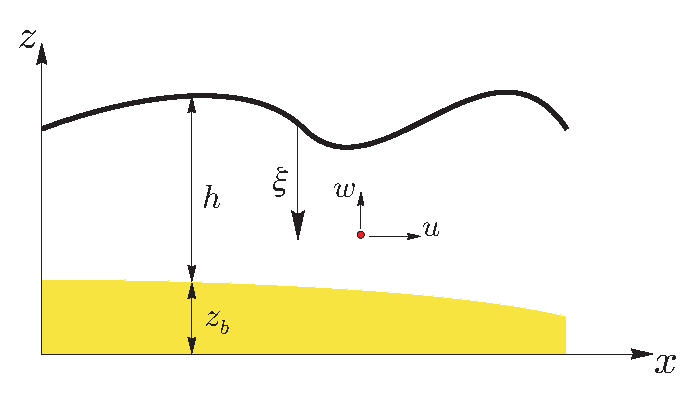
\includegraphics[width=7.0cm]{one-dimensional-axis_Serre.eps}
\end{center}
\caption{The notation used for one-dimensional flow governed by the Serre equation.}
\label{fig:Notation}
\end{figure}
In addition to the above equations, a number of boundary conditions must be satisfied. These are;
\begin{subequations}\label{eq:Seabra_all}
%\begin{enumerate}[(a)]
\begin{itemize}
\item the kinematic condition at the free surface $(z = h + z_b)$,
\begin{linenomath*}
\begin{equation}
w|_{h+z_b} = \dfrac{\partial h}{\partial t} + u \dfrac{\partial (h + z_b)}{\partial x},
\end{equation}
\end{linenomath*}
\item the kinematic condition at the bed $(z = z_b)$
\begin{linenomath*}
\begin{equation}
w|_{z_b} = u \dfrac{\partial z_b}{\partial x},
\end{equation}
\end{linenomath*}
\item the dynamic condition at the surface $(z = h + z_b)$
\begin{linenomath*}
\begin{equation}
p(\xi = 0) = p_a.
\end{equation}
\end{linenomath*}
\end{itemize}
%\end{enumerate}
\end{subequations}
This is the atmospheric pressure at the water surface, usually taken to be $p_a = 0$.

The three-dimensional problem can be reduced to a two-dimensional problem in $(x,y)$ by incorporating the vertical velocity of the fluid particles with additional higher-order terms in the $x$- and $y$-momentum equations. For example, in the $x$-direction, this can be achieved by choosing the horizontal velocity variable, $u(x,z,t)$ or the functional form of the variation of $u(x,z,t)$ with depth.  The choice of horizontal velocity variable, $u(x,z,t)$ to be used, results in a variety of equations with different forms and different dispersion characteristics \cite{Madsen-etal-1991-371,Beji-Nadaoka-1996,Madsen-Sorensen-1992-183,Witting-J-1984-203,Zou-Z-1999-767}. It has been shown by \citeN{Mei-etal-2005} and \citeN{Nwogu-O-1993-618} that the accuracy of linear dispersion characteristics is dependent on the choice of the velocity variable. The choice of velocity variable is not unique. In the derivation of the Serre equation, instead of using the velocity at a particular depth, the point velocity in the $x$-direction is assumed to be uniform over the water depth, so that $u(x,z,t) = \bar{u}(x,t)$. This assumption is not necessary for the derivation of the continuity equation. If the depth-averaged velocity in the $x$-direction, given by
\begin{linenomath*}
\begin{gather*}
\bar{u} = \dfrac{1}{h} \int_{z_b}^{h+z_b} u(x,z,t) \, dz
\end{gather*}
\end{linenomath*}
is used, then the continuity equation
\begin{linenomath*}
\begin{gather}
\dfrac{\partial h}{\partial t} + \bar{u} \dfrac{\partial h}{\partial x} +  h \dfrac{\partial \bar{u}}{\partial x} = 0 %
\label{eq:Boussinsq_continuity}
\end{gather}
\end{linenomath*}
where $h$ and $\bar{u}$ are the primitive variables, is exact.

From \eqref{eq:Euler_continuity} it follows that the vertical velocity at any depth $z - z_b$ is given by
\begin{linenomath*}
\begin{gather}
w |_z = -(z - z_b) \dfrac{\partial \bar{u}}{\partial x}
\label{eq:depth-averaged}
\end{gather}
\end{linenomath*}
for a horizontal bed. The vertical velocity is a linear function of the water depth, zero at the bed and a maximum at the water surface. The shallow water wave equations assume that $w|_z = 0$.

Integrating the point quantities in \eqref{eq:Euler_momentum_x} over the flow depth $z_b$ to $h+z_b$, and satisfying \eqref{eq:Seabra_all} produces the one-dimensional $x$-momentum equations
\begin{linenomath*}
\begin{gather}
\dfrac{\partial \bar{u}}{\partial t} + \bar{u} \dfrac{\partial \bar{u}}{\partial x} + \dfrac{1}{h}\dfrac{\partial}{\partial x} \left [  \dfrac{gh^2}{2} + \dfrac{h^3}{3} \left ( \dfrac{\partial \bar{u}}{\partial x} \dfrac{\partial \bar{u}}{\partial x} - \bar{u} \dfrac{\partial^2\bar{u}}{\partial x^2} - \dfrac{\partial^2\bar{u}}{\partial x \partial t} \right ) \right ] = 0
\label{eq:Boussinsq_momentum}
\end{gather}
\end{linenomath*}
Equation \eqref{eq:Boussinsq_momentum} contain a third-order spatial derivative term and has the form of a dispersion equation. This term can severely restrict the time step that can be used if standard explicit finite difference schemes are used to solve these equations.

Multiplying \eqref{eq:Boussinsq_momentum} by $h$, adding \eqref{eq:Boussinsq_continuity} pre-multiplied by $\bar{u}$ and making use of \eqref{eq:Boussinsq_continuity} to obtain;
\begin{linenomath*}
\begin{subequations}\label{eq:Serre_conservative_form}
\begin{gather}
\dfrac{\partial h}{\partial t} + \dfrac{\partial (\bar{u}h)}{\partial x} = 0
\label{eq:Serre_continuity}
\end{gather}
and
\begin{gather}
\underbrace{\underbrace{\dfrac{\partial (\bar{u}h)}{\partial t} + \dfrac{\partial}{\partial x} \left ( \bar{u}^2h + \dfrac{gh^2}{2}\right )}_{\text{Shallow Water Wave Equations}} + \underbrace{\dfrac{\partial}{\partial x} \left (  \dfrac{h^3}{3} \left [ \dfrac{\partial \bar{u} }{\partial x} \dfrac{\partial \bar{u}}{\partial x} - \bar{u} \dfrac{\partial^2 \bar{u}}{\partial x^2}  - \dfrac{\partial^2 \bar{u}}{\partial x \partial t}\right ] \right )}_{\text{Dispersion Terms}} = 0.}_{\text{Serre Equations}}
\label{eq:Serre_momentum}
\end{gather}
\end{subequations}
\end{linenomath*}
which is written in terms of the conservative variables, $h$ and $\bar{u}h$. The terms in the square parenthesis are the dispersive terms which contain high order spatial derivative terms and a mixed spatial and temporal derivative term. This is generally the case for dispersive equations, with the exception of the Boussinesq equation \cite{Basco-D-1987}, where the momentum equation is given by
\begin{linenomath*}
\begin{gather}
\dfrac{\partial (\bar{u}h)}{\partial t} + \dfrac{\partial}{\partial x} \left ( \bar{u}^2h + \dfrac{gh^2}{2}\right ) - \dfrac{h^3}{3} \dfrac{\partial^3 \bar{u}}{\partial x^2 \partial t} = 0.
\end{gather}
\end{linenomath*}
the product derivative and third-order space derivative terms in \eqref{eq:Serre_momentum} are ignored.

The dispersive terms influence the pressure distribution in the water column, which is given by
\begin{linenomath*}
\begin{gather}\label{eq:pressure_serre}
p|_\xi = p_a + \rho g \xi + \dfrac{\rho}{2} \xi ( 2h - \xi ) \left ( \dfrac{\partial \bar{u}}{\partial x} \dfrac{\partial \bar{u}}{\partial x} - \bar{u} \dfrac{\partial^2 \bar{u}}{\partial x^2} -  \dfrac{\partial^2 \bar{u}}{\partial x \partial t} \right ).
\end{gather}
\end{linenomath*}
It is less than the hydrostatic pressure,  $p(\xi) = \rho g \xi$ at the crest of a wave and greater than the hydrostatic pressure distribution at the troughs. Ignoring all the dispersive terms in \eqref{eq:Serre_momentum} results in the well known nonlinear shallow water wave equations, where the pressure distribution is hydrostatic.

Equation \eqref{eq:Serre_conservative_form} are known as the Serre equations \cite{Serre-F-1953-857,Seabra-Santos-etal-1987-117,Carter-Cienfuegos-2010-259} and unlike some Boussinesq-type equations, they retain full nonlinearity in the dispersive terms \cite{El-etal-2006}. They have been derived by Serre \cite{Serre-F-1953-857}, Su and Gardner \cite{Su-Gardener-1969-536} and Seabra-Santos \emph{et al.} \cite{Seabra-Santos-etal-1987-117} and are equivalent to the depth averaged Green and Naghadi \cite{Green-Naghdi-1976-237} equations. They are considered to be good approximations to the full Euler equations up to a wave breaking \cite{Bonneton-etal-2011-1479,Bonneton-etal-2011-589}. Unlike the shallow water wave equations, which are hyperbolic for finite water depth, although they are evolution-type equations, the Serre equations are neither hyperbolic or parabolic.

The major differences between the Serre and shallow water wave equations are summarized in Table \ref{The major differences in the derivation of the Serre and Shallow water wave equations}.

%--------------------------------------------------------------------------------
\section{Alternative Conservation Law Form of the Sere Equations}
\label{section:Alternative Conservation Law Form of the Sere Equations}
%--------------------------------------------------------------------------------

We could solve the Serre equations using a variety of methods. However, if we can write the equations in conservation law form, then there are very efficient schemes for solving conservation laws which could be used to solve the Serre equations. These schemes are capable of handling step gradients in a problem with potentially a significant saving in computational effort if the Serre equations can be written in conservation law form.

For example, using a simple explicit finite difference schemes, stability analysis of simple explicit finite differences scheme for the advection equation (conservation law form)
\begin{linenomath*}
\begin{gather*}
\dfrac{\partial q}{\partial t} + \dfrac{\partial q}{\partial x} = 0,  \qquad \Delta t \le \Delta x
\end{gather*}
\end{linenomath*}
would show that the computational time step is proportional to the computation distance step. For the diffusion equation
\begin{linenomath*}
\begin{gather*}
\dfrac{\partial q}{\partial t} - \dfrac{\partial^2 q}{\partial x^2} = 0, \qquad \Delta t \le \Delta x^2/2
\end{gather*}
\end{linenomath*}
the computational time step is proportional to $\Delta x^2$ and for the dispersion equation
\begin{linenomath*}
\begin{gather*}
\dfrac{\partial q}{\partial t} + \dfrac{\partial^3 q}{\partial x^3} = 0 \qquad \Delta t \le \Delta x^3/2
\end{gather*}
\end{linenomath*}
the time step is proportional to $\Delta x^3$. Potentially there is considerable savings to be made if the Serre equations can be written in conservation law form.

The flux term in the momentum equation, \eqref{eq:Serre_momentum} contains a mixed spatial and temporal derivative term which is difficult to treat numerically. It is possible to replace this term by a combination of spatial and temporal derivative terms.

Consider
\begin{linenomath*}
\begin{gather*}
\dfrac{\partial^2}{\partial x \partial t} \left ( \dfrac{h^3}{3} \dfrac{\partial \bar{u}}{\partial x} \right ) = \dfrac{\partial }{\partial t} \left ( h^2 \dfrac{\partial h}{\partial x} \dfrac{\partial \bar{u}}{\partial x} + \dfrac{h^3}{3} \dfrac{\partial^2 \bar{u}}{\partial x^2} \right ) =
\dfrac{\partial }{\partial x} \left ( h^2 \dfrac{\partial h}{\partial t} \dfrac{\partial \bar{u}}{\partial x} + \dfrac{h^3}{3} \dfrac{\partial^2 \bar{u}}{\partial x \partial t} \right ).
\end{gather*}
\end{linenomath*}
Rearranging then
\begin{linenomath*}
\begin{gather*}
\dfrac{\partial }{\partial x} \left ( \dfrac{h^3}{3} \dfrac{\partial^2 \bar{u}}{\partial x \partial t} \right ) = \dfrac{\partial }{\partial t} \left ( h^2 \dfrac{\partial h}{\partial x} \dfrac{\partial \bar{u}}{\partial x} + \dfrac{h^3}{3} \dfrac{\partial^2 \bar{u}}{\partial x^2} \right ) - \dfrac{\partial }{\partial x} \left ( h^2 \dfrac{\partial h}{\partial t} \dfrac{\partial \bar{u}}{\partial x}\right ).
\end{gather*}
\end{linenomath*}
Making use of the continuity equation, \eqref{eq:Serre_continuity}
\begin{linenomath*}
\begin{gather*}
\dfrac{\partial }{\partial x} \left ( \dfrac{h^3}{3} \dfrac{\partial^2 \bar{u}}{\partial x \partial t} \right ) = \dfrac{\partial }{\partial t} \left ( h^2 \dfrac{\partial h}{\partial x} \dfrac{\partial \bar{u}}{\partial x} + \dfrac{h^3}{3} \dfrac{\partial^2 \bar{u}}{\partial x^2} \right ) + \dfrac{\partial }{\partial x} \left [ h^2 \dfrac{\partial \bar{u}}{\partial x} \left ( \bar{u}\dfrac{\partial h}{\partial x} + h \dfrac{\partial \bar{u}}{\partial x}  \right ) \right ]
\end{gather*}
\end{linenomath*}
and the momentum equation, \eqref{eq:Serre_momentum} becomes
\begin{linenomath*}
\begin{gather*}
\dfrac{\partial }{\partial t} \left ( \bar{u}h -  h^2 \dfrac{\partial h}{\partial x} \dfrac{\partial \bar{u}}{\partial x} - \dfrac{h^3}{3} \dfrac{\partial^2 \bar{u}}{\partial x^2}  \right ) + \dfrac{\partial}{\partial x} \left ( \bar{u}^2h + \dfrac{gh^2}{2} - \bar{u}h^2 \dfrac{\partial h}{\partial x}\dfrac{\partial \bar{u}}{\partial x} - \dfrac{\bar{u}h^3}{3} \dfrac{\partial^2 \bar{u}}{\partial x^2} - \dfrac{2h^3}{3}\dfrac{\partial \bar{u}}{\partial x}\dfrac{\partial \bar{u}}{\partial x} \right ) \nonumber  = 0.
\end{gather*}
\end{linenomath*}
The momentum equation can be written in terms of a new conservative quantity as
\begin{linenomath*}
\begin{gather}\label{eq:G_momentum}
\dfrac{\partial G}{\partial t} + \dfrac{\partial }{\partial x} \left ( G\bar{u} + \dfrac{gh^2}{2} - \dfrac{2 h^3}{3} \dfrac{\partial \bar{u}}{\partial x} \dfrac{\partial \bar{u}}{\partial x} \right ) = 0
\end{gather}
\end{linenomath*}
where the new conserved quantity, $G$ is given by the second-order elliptic equation
\begin{linenomath*}
\begin{gather}\label{eq:G}
G = \bar{u}h - h^2 \dfrac{\partial h}{\partial x} \dfrac{\partial \bar{u}}{\partial x} - \frac{h^3}{3} \dfrac{\partial^2 \bar{u}}{\partial x^2}
\end{gather}
\end{linenomath*}
which can be written in divergent form as
\begin{linenomath*}
\begin{gather}\label{eq:G_divergent}
G = \bar{u}h - \dfrac{\partial }{\partial x} \left ( \dfrac{h^3}{3} \dfrac{\partial \bar{u}}{\partial x} \right ).
\end{gather}
\end{linenomath*}
The temporal derivative in the momentum equation has been eliminated from the flux term. In contrast to \eqref{eq:Serre_conservative_form}, the flux term now only contains spatial derivatives. The quantity, $G/h$ is known as irrotationality \cite{Carter-Cienfuegos-2010-259} or potential vorticity \cite{Dias-Milewski-2010}. The quantity $G$ is a new conserved variable that is admissible to the Serre equation. The Serre equations also admit the conservation of mass, momentum, energy and irrotationality \cite{Bonneton-etal-2011-1479,Carter-Cienfuegos-2010-259}. For smooth problems, all of these equations and \eqref{eq:G_momentum} will produce identical solutions.

The alternative form of the Serre equations can be written in vector form as
\begin{linenomath*}
\begin{subequations}\label{eq:Serre_Vector}
\begin{gather}\label{eq:Serre_advection_equation}
\dfrac{\partial \mathbf{U}(x,t)}{\partial t} + \dfrac{\partial \mathbf{F}(\mathbf{U}(x,t))}{\partial x} = 0.
\end{gather}
where,
\begin{gather}\label{eq:Serre_conserved_quantity}
\textbf{U}(x,t) = \left[ \begin{array}{c} h \\ G
\end{array} \right],
\end{gather}
and
\begin{gather}\label{eq:Serre_flux}
\textbf{F}(\textbf{U}(x,t)) = \left [ \begin{array}{c} f(1) \\
f(2) \end{array} \right ] = \left[ \begin{array}{c} \bar{u}h \\
G\bar{u} + \dfrac{gh^2}{2} - \dfrac{2h^3}{3} \dfrac{\partial
\bar{u}}{\partial x} \dfrac{\partial \bar{u}}{\partial x}
\end{array} \right].
\end{gather}
\end{subequations}
\end{linenomath*}

%--------------------------------------------------------------------------------
\subsection{Properties of the modified Serre equations}
%--------------------------------------------------------------------------------

The Serre equations have two identical pairs of characteristics with slopes
\begin{linenomath*}
\begin{gather*}
\dfrac{dx}{dt} = \bar{u}, \bar{u} \quad\text{and} \quad \dfrac{dx}{dt} = \infty, \infty.
\end{gather*}
\end{linenomath*}
They are not hyperbolic and do not have any Riemann invariants. However, useful properties of the Serre equations,  \eqref{eq:Serre_conservative_form} or \eqref{eq:Serre_Vector} can be obtained by applying the Fourier analysis to the linearized equations and observing the behaviour of a harmonic wave of the form
\begin{linenomath*}
\begin{gather}\label{eq:Fourier_components}
h(x,t) = A e^{i(kx - \omega t)} \quad \text{and} \quad u(x,t) = U e^{i(kx - \omega t)}
\end{gather}
\end{linenomath*}
where $A$ and $U$ are unknown coefficients, $\omega$ is the frequency, $k$ the wave number and $i = \sqrt{-1}$.

The linearized Serre equations are obtained by assuming that  the solution of $\bar{u}(x,t)$ and $h(x,t)$ can be expressed as
\begin{linenomath*}
\begin{subequations}\label{eq:purturbed_variables}
\begin{gather}
h(x,t) = h_0(x,t) + \epsilon h_1(x,t) + \epsilon^2 h_2(x,t) + \cdots
\end{gather}
and
\begin{gather}
\bar{u}(x,t) = u_0(x,t) + \epsilon u_1(x,t) + \epsilon^2 u_2(x,t) + \cdots
\end{gather}
\end{subequations}
\end{linenomath*}
where $u_0$, $u_1$, $\ldots$, $h_0$, $h_1$, $\ldots$ are to be determined.

Using \eqref{eq:purturbed_variables}, then the continuity equation, \eqref{eq:Serre_continuity} becomes, to terms of up to order $\epsilon$
\begin{linenomath*}
\begin{subequations}\label{eq:linearized_Serre}
\begin{gather}\label{eq:linearized_Serre_continuity}
\dfrac{\partial h_1}{\partial  t} + h_0 \dfrac{\partial u_1}{\partial x} +  u_0 \dfrac{\partial h_1}{\partial x} = 0
\end{gather}
and for the momentum equation, \eqref{eq:Serre_momentum}
\begin{gather}\label{eq:linearized_Serre_momentum}
\dfrac{\partial u_1}{\partial t} +  g \dfrac{\partial h_1}{\partial x} + u_0 \dfrac{\partial u_1}{\partial x} -  \dfrac{h_0^2}{3} \left ( u_0 \dfrac{\partial^3 u_1}{\partial x^3}  + \dfrac{\partial^3 u_1}{\partial x^2 \partial t} \right )  = 0
\end{gather}
which makes use of the linearized  continuity equation.
\end{subequations}
\end{linenomath*}

Substituting \eqref{eq:Fourier_components}, the linearized equations become
\begin{linenomath*}
\begin{subequations}
\begin{gather}
-A \omega + u_0 A k + h_0 U k = 0,
\end{gather}
and
\begin{gather}
- U \omega +  g A k +  u_0 U k - \dfrac{1}{3} h_0^2 U  \omega k^2 + \dfrac{1}{3} h_0^2 u_0 U  k^3 = 0.
\end{gather}
\end{subequations}
\end{linenomath*}
For a nontrivial solution
\begin{linenomath*}
\begin{gather*}
\left|
  \begin{array}{cc}
     -\omega + u_0 k & h_0 k \\
    g k & -\omega + u_0 k - \dfrac{1}{3} h_0^2 \omega k^2 + \dfrac{1}{3} h_0^2 u_0 k^3 \\
  \end{array}
\right| = 0
\end{gather*}
\end{linenomath*}
or
\begin{linenomath*}
\begin{gather*}
\omega_{1,2} = u_0 k \pm k \sqrt{g h_0} \sqrt{\dfrac{3}{\mu^2 + 3}} \nonumber
\end{gather*}
\end{linenomath*}
where $\mu = h_0k$ is the frequency dispersion. The dispersive terms have no effect on $u_0$, only on the celerity of a small disturbance.

For non-dispersive waves, the phase velocity, $\upsilon_p = \text{Re}(\omega)/k$ is identical to the group velocity $\upsilon_g = d\text{Re}(\omega)/dk$. This is the case for the shallow water wave equation where, $\upsilon_p = \upsilon_g = u_0 \pm \sqrt{gh_0}$. The phase speed is independent of the wave number, $k$ and all wave components travel at the same speed, $u_0 \pm \sqrt{g h_0}$. This is not the case for the Serre equation, where the phase speed is
\begin{linenomath*}
\begin{subequations}
\label{eq:wave_speeds_Serre_equations}
\begin{gather}
\upsilon_p = u_0 \pm \sqrt{gh_0}\sqrt{\dfrac{3}{\mu^2 + 3}}
\end{gather}
and the group velocity is
\begin{gather}
\upsilon_g = u_0 \pm \sqrt{gh_0}\left ( \sqrt{\dfrac{3}{\mu^2 + 3}} \mp \mu^2 \sqrt{\dfrac{3}{(\mu^2 + 3)^3}} \right ) \neq \upsilon_p.
\end{gather}
\end{subequations}
\end{linenomath*}
Both are dependent on the wave number, $k$. Since the group speed is slower than the phase speed, the Serre equations describe dispersive waves. This is a characteristic of dispersive waves, the group and phase speeds differ.

\begin{table}[t]
\caption{The major differences between the Serre and shallow water wave equations describing one-dimensional unsteady flow over a frictionless horizontal bed.}
\label{The major differences in the derivation of the Serre and Shallow water wave equations}
\centering
{\footnotesize
\begin{tabular}{lcc}
\phantom{p} & \\
\hline
\phantom{p} & \\
& \textbf{Serre Equations} & \textbf{Shallow Water Wave Equations} \\
\phantom{p} & \\
\hline
\phantom{p} & \\
Longitudinal velocity & $\bar{u}(x,t) = u(x,t)$ & $\bar{u}(x,t) = \dfrac{1}{h} \displaystyle\int_0^h u(x,z,t) \, dz$ \\
\phantom{p} & \\
Vertical particle velocity & $w|_z = -(z - z_b) \dfrac{\partial \bar{u}}{\partial x}$ & $w|_z = 0$ \\
\phantom{p} & \\
Pressure  & $p|_{\xi} = p_a + \rho g \xi + \dfrac{\rho}{2} \xi ( 2h - \xi ) \left ( \dfrac{\partial \bar{u}}{\partial x} \dfrac{\partial \bar{u}}{\partial x} - \bar{u} \dfrac{\partial^2 \bar{u}}{\partial x^2} -  \dfrac{\partial^2 \bar{u}}{\partial x \partial t} \right )  $ & $p|_{\xi} = p_a + \rho g\xi$ \\
\phantom{p} & \\
Continuity equation & $\dfrac{\partial h}{\partial t} + \dfrac{\partial (\bar{u}h)}{\partial x} = 0$ & $\dfrac{\partial h}{\partial t} + \dfrac{\partial (\bar{u}h)}{\partial x} = 0$ \\
\phantom{p} & \\
Momentum equation & $\dfrac{\partial (\bar{u}h)}{\partial t} + \dfrac{\partial}{\partial x} \left [  \bar{u}^2h + \dfrac{gh^2}{2} + \dfrac{h^3}{3} \left ( \dfrac{\partial \bar{u}}{\partial x} \dfrac{\partial \bar{u}}{\partial x} - \bar{u} \dfrac{\partial^2 \bar{u}}{\partial x^2} - \dfrac{\partial^2 \bar{u}}{\partial x \partial t} \right ) \right ] = 0$ & $\dfrac{\partial (\bar{u}h)}{\partial t} + \dfrac{\partial}{\partial x} \left ( \bar{u}^2h + \dfrac{gh^2}{2}\right ) = 0$ \\
\phantom{p} & \\
Phase velocity & $v_p = \bar{u} \pm \sqrt{gh} \sqrt{\dfrac{3}{\mu^2 + 3}}$ & $v_p = \bar{u} \pm \sqrt{gh}$ \\
\phantom{p} & \\
Group velocity & $v_g = \bar{u} \pm \sqrt{gh} \left ( \sqrt{\dfrac{3}{\mu^2 + 3}} \mp \mu^2 \sqrt{\dfrac{3}{(\mu^2 + 3)^3}} \right ) $ & $v_g = \bar{u} \pm \sqrt{gh}$ \\
\phantom{p} & \\
\hline
\end{tabular}
}
\end{table}

%--------------------------------------------------------------------------------
\section{Solving the Serre Equations Written in Conservation Law Form}
\label{section:Solving the Serre Equations Written in Conservation Law Form}
%--------------------------------------------------------------------------------

The Serre equations is solved using a second-order finite volume method. In a finite volume method the solution to a conservation law, \eqref{eq:Serre_advection_equation} is advanced by solving
\begin{linenomath*}
\begin{gather}
\dfrac{\partial \mathbf{U}_j}{\partial t} + \dfrac{1}{V_j} \oint_{S_j} \mathbf{F}(\mathbf{U}) \cdot \vec{\mathbf{u}} \, ds = 0
\label{eq:finite_volume_method_Vector}
\end{gather}
\end{linenomath*}
where $S_j$ is the surface area of element $I_j$, $V_j$ is the volume of the element $I_j$ and $\vec{\mathbf{u}}$ is the unit vector normal to the surface of element $I_j$ pointing outward. In one-dimension, the cells are line segments $I_j = [x_{j-1/2},x_{j+1/2}]$ that are assumed to be uniform in space. Then \eqref{eq:finite_volume_method_Vector} can be written in semi-discrete form as
\begin{linenomath*}
\begin{gather}\label{eq:semi-discrete}
\dfrac{d\bar{q}_j(t)}{dt} = \mathcal{L}(\bar{q}(x,t)) = \dfrac{f(\bar{q}(x_{j+1/2},t)) - f(\bar{q}(x_{j-1/2},t))}{\Delta x}
\end{gather}
\end{linenomath*}
for a conserved quantity, $q(x,t)$ where $\Delta x = x_{j+1/2} - x_{j-1/2}$, $x_j = (x_{j+1/2} + x_{j-1/2})/2$.

In the discrete forms of \eqref{eq:finite_volume_method_Vector}, $f(q(x_{j \pm 1/2},t)) = f_{j \pm 1/2}(q_{j-1}(t), \dots, q_{j+1}(t)) = F_{j \pm 1/2}$ represents the numerical approximation of the physical flux $f(q(x,t))$ of the conserved quantity, $q(x,t)$ across the boundary of cell $I_j$ at $x_{j \pm 1/2}$ at time $t$, and
\begin{linenomath*}
\begin{gather}\label{eq:depth_average_velocity}
\bar{q}_j(t) = \dfrac{1}{\Delta x} \int_{x_{j-1/2}}^{x_{j+1/2}} q(x,t) \, dx
\end{gather}
\end{linenomath*}
is the average value of the state variable, $q(x,t)$ in $I_j$ at time $t$. Equation \eqref{eq:depth_average_velocity} ensures that mass is conserved in each cell.

The flux , $F_{j+1/2}$ is a function of the left and right extrapolated state values $q^+_{j+1/2}$ and $q^-_{j+1/2}$, obtained from piecewise polynomials passing through consecutive values of $\bar{q}_j$. Therefore,
\begin{linenomath*}
\begin{gather*}
F_{j+1/2} = f_{j+1/2}(q_{j+1/2}^+,q_{j+1/2}^-).
\end{gather*}
\end{linenomath*}
At the cell interface generally, $q^+_{j+1/2} \ne q^-_{j+1/2}$ and a local Riemann problem is solved to obtain the flux between the cells.

The overall accuracy of the numerical scheme is dependent on the accuracy of the reconstruction method and the order of accuracy of the time integration of the semi-discrete system, \eqref{eq:semi-discrete}.

%--------------------------------------------------------------------------------
\subsection{Reconstruction}
%--------------------------------------------------------------------------------

To achieve second-order, $\mathcal{O}(\Delta x^2)$ accuracy a linear polynomial, $P_j(x) = a_j + b_j(x - x_j)$ is fitted through the cell averages. The reconstructed cell interface values are given by
\begin{linenomath*}
\begin{subequations}\label{eq:linear_reconstruction}
\begin{gather}
q^-_{j+1/2} = \bar{q}_j + \phi(r_j) \dfrac{\bar{q}_j - \bar{q}_{j-1}}{2}
\end{gather}
and
\begin{gather}
q^+_{j-1/2} = \bar{q}_j - \phi(r_j) \dfrac{\bar{q}_j - \bar{q}_{j-1}}{2}
\end{gather}
\end{subequations}
\end{linenomath*}
where
\begin{linenomath*}
\begin{gather*}
r_j = \dfrac{\bar{q}_j - \bar{q}_{j-1}}{\bar{q}_{j+1} - \bar{q}_j} = \dfrac{\Delta \bar{q}_{j-1/2}}{\Delta \bar{q}_{j+1/2}}
\end{gather*}
\end{linenomath*}
and $\phi(r_j)$ is a nonlinear constraints imposed on the reconstruction to ensures that the scheme remains \emph{TVD} and second-order away from extremes, where $r < 0$.  The nonlinear limiter prevents unwanted oscillations and ensures that the results are physical (bounded) and therefore stable.

An example of a non-linear limiter is the \emph{generalized
minmod} limiter \cite{vanLeer-B-1979-101}
\begin{linenomath*}
\begin{gather*}
\phi(\bar{q},\theta) = \text{minmod} \left ( \theta \Delta \bar{q}_{j-1/2}, (\Delta \bar{q}_{j+1/2} + \Delta \bar{q}_{j-1/2})/2, \theta \Delta \bar{q}_{j+1/2} \right ), \quad 1 \leq \theta \leq 2,
\end{gather*}
\end{linenomath*}
where
\begin{linenomath*}
\begin{eqnarray*}
\textrm{minmod}(x_1,x_2,x_3,...) = \left \lbrace
\begin{array}{cl}
\underset{j}{\min}(x_j) & \text{if} \,\, x_j > 0, \,\, \forall j, \\
\underset{j}{\max}(x_j) & \text{if} \,\, x_j < 0, \,\, \forall j, \\
0 & \text{otherwise}.
\end{array}
\right .
\end{eqnarray*}
\end{linenomath*}
The parameter $\theta$ controls the amount of diffusion in the numerical scheme. When a local extrema has been encountered, $r_j \le 0$ and $\phi(r_j) = 0$. In this case the reconstruction reverts to a piecewise constant reconstruction. In smooth regions, $r_j \rightarrow 1$ and $\phi(r_j) \rightarrow 1$ and the reconstruction is first-order producing a second-order accurate scheme.

%--------------------------------------------------------------------------------
\subsection{Local Riemann Problem} %
%--------------------------------------------------------------------------------

The reconstruction of the conserved quantities, $\bar{q}^\pm_{j \pm 1/2}$ at the cell interface from the cell averages $\bar{q}_j$ will generally result in a discontinuity in these quantities at the cell interface.

The flux of material across the interface of a cell is estimated by solving the local Riemann problem, defined by the initial value problem
\begin{linenomath*}
\begin{gather*}
\bar{q}(x_{j+1/2}) = \left \lbrace \begin{matrix} q_{j+1/2}^+ \;\; \text{if} \;\; x < x_{j+1/2} \\
q_{j+1/2}^- \;\; \text{if} \;\; x > x_{j+1/2}.
\end{matrix}
\right .
\end{gather*}
\end{linenomath*}
The numerical approximation of the physical flux across the boundary of cell, $F_{j+1/2}$ is given by the explicit upwind central scheme proposed by Kurganov \emph{et al.} \cite{Kurganov-etal-2001-707} as
\begin{linenomath*}
\begin{gather}\label{eq:HLL_flux}
F_{j+1/2} = \dfrac{a_{j+1/2}^+ f(q^-_{j+1/2}) -a_{j+1/2}^- f(q^+_{j+1/2})}{a^+_{j+1/2} - a^-_{j+1/2}}  + \dfrac{a_{j+1/2}^+ \, a_{j+1/2}^-}{a_{j+1/2}^+ - a_{j+1/2}^-} \left [ q^+_{j+1/2} - q^-_{j+1/2} \right ].
\end{gather}
\end{linenomath*}
where the spatial derivatives in the second component of the flux term, \eqref{eq:Serre_flux} are evaluated using first-order upwind differencing, so that
\begin{linenomath*}
\begin{subequations}
\begin{gather}
f(G^+_{j+1/2}) = (\bar{u}G)^+_{j+1/2} + \dfrac{g{h^+_{j+1/2}}^2}{2} - \dfrac{2{h^+_{j+1/2}}^3}{3\Delta x^2} \left ( u^+_{j+3/2} - u^+_{j+1/2} \right )^2
\end{gather}
\begin{gather}
f(G^-_{j+1/2}) = (\bar{u}G)^-_{j+1/2} + \dfrac{g{h^-_{j+1/2}}^2}{2} - \dfrac{2{h^-_{j+1/2}}^3}{3\Delta x^2} \left ( u^-_{j+1/2} - u^-_{j-1/2} \right )^2
\end{gather}
\end{subequations}
\end{linenomath*}
and for the first component of the flux term, it is simply; $f(h^\pm_{j+1/2}) = (\bar{u}h)^\pm_{j+1/2}$.

At the interface of a cell, $x_{j \pm 1/2}$ a discontinuity in the state variable will propagate with right- and left-sided local speeds, which are estimated by
\begin{linenomath*}
\begin{subequations}
\label{eq:shock_speeds}
\begin{gather*}
a^+_{j+1/2} = \text{max}\left [ \lambda_2(q_{j+1/2}^-), \, \lambda_2(q_{j+1/2}^+), \, 0 \right ],
\end{gather*}
and
\begin{gather*}
a^-_{j+1/2} = \text{min}\left [ \lambda_1 (q_{j+1/2}^-), \, \lambda_1 (q_{j+1/2}^+), \,0 \right ]
\end{gather*}
\end{subequations}
\end{linenomath*}
where $\lambda_1$ and $\lambda_2$ are estimates of the smallest and largest eigenvalues, respectively  of the Jacobian $\partial f(\mathbf{u})/\partial \mathbf{u}$ which correspond to the phase speeds. This is a common feature of this and other exact Riemann or approximate Riemann solvers. The wave speeds or an estimate of the wave speed is required (see, for example Zoppou and Roberts \cite{Zoppou-Roberts-2003-11}).

%--------------------------------------------------------------------------------
\subsubsection{Propagation Speeds of a Local Shock} %
%--------------------------------------------------------------------------------

As the wave number approaches infinity, $k \rightarrow \infty$, from \eqref{eq:wave_speeds_Serre_equations} the phase and group speeds of the Serre equations,  $v_p \rightarrow v_g \rightarrow u_0 \pm \sqrt{g h_0}$, are equal to the phase speed of shallow water waves. Indeed the phase speed for the Serre equations are bounded
\begin{linenomath*}
\begin{gather*}
u_0 - \sqrt{g h_0} \le u_0 \pm \sqrt{gh_0}\sqrt{\dfrac{3}{k^2h^2 + 3}} \le u_0 + \sqrt{g h_0}
\end{gather*}
\end{linenomath*}
by the phase speed of the shallow water wave equations. We now have an estimate of the maximum and minimum shock speed required by our chosen approximate Riemann solver.

%--------------------------------------------------------------------------------
\subsection{Strong-Stability-Preserving Runge-Kutta Scheme} %
%--------------------------------------------------------------------------------

Time integration of the semi-discrete system \eqref{eq:semi-discrete} is performed using a second-order Strong Stability Preserving (\emph{SSP}) Runge-Kutta scheme. Strong stability preserving schemes involve a convex combination of first-order forward Euler steps that preserve the desirable Total Variational Diminishing (\emph{TVD}) properties of the Euler scheme \cite{Shu-Osher-1988-439,Gottlieb-etal-2009-251}.

A second-order two-stage strong stability preserving Runge-Kutta scheme is given by \cite{Shu-Osher-1988-439,MacDonald-etal-2008-89}
\begin{linenomath*}
\begin{subequations}
\begin{gather}
\bar{q}^{(1)} = \bar{q}^n - \Delta t \mathcal{L}(t_n,\bar{q}^n),
\end{gather}
\begin{gather}
\bar{q}^{(2)} = \bar{q}^{(1)} - \Delta t \mathcal{L}(t_{n+1},\bar{q}^{(1)}),
\end{gather}
and
\begin{gather}
\bar{q}^{n+1} = \dfrac{1}{2}\bar{q}^n + \dfrac{1}{2}\bar{q}^{(2)}.
\end{gather}
\label{eq:RK_TVD_shu_Osher0}
\end{subequations}
\end{linenomath*}

%--------------------------------------------------------------------------------
\subsection{Solution Process} %
%--------------------------------------------------------------------------------

The solution of the Serre equations involves the following steps
\begin{linenomath*}
\begin{gather}
\underbrace{\left [
          \begin{array}{c}
            h \\
            G \\
          \end{array}
        \right ]^n \stackrel{\mathcal{A}}{\longrightarrow} \bar{u}^n}_{\text{\ding{192}}} \rightarrow \underbrace{\left [
          \begin{array}{c}
            h \\
            G \\
          \end{array}
        \right ]^{(1)}
        = \left [
          \begin{array}{c}
            h \\
            G \\
          \end{array}
        \right ]^{n} - \Delta t \mathcal{L} \left [
          \begin{array}{c}
            h \\
            G \\
          \end{array}
        \right ]^{n}}_{\text{\ding{193} First Euler Step}} \nonumber \\
\underbrace{ \left [ \begin{array}{c}
            h \\
            G \\
          \end{array}
        \right ]^{(1)} \stackrel{\mathcal{A}}{\longrightarrow} \bar{u}^{(1)}}_{\text{ \ding{194}}} \rightarrow
        \underbrace{ \left [ \begin{array}{c}
            h \\
            G \\
          \end{array}
        \right ]^{(2)}
         = \left [
          \begin{array}{c}
            h \\
            G \\
          \end{array}
        \right ]^{(1)} - \Delta t \mathcal{L} \left [
          \begin{array}{c}
            h \\
            G \\
          \end{array}
        \right ]^{(1)}}_{\text{\ding{195} Second Euler Step}} \nonumber \\
  \underbrace{\left [
          \begin{array}{c}
            h \\
            G \\
          \end{array}
        \right ]^{n+1}
         = \dfrac{1}{2}\left [
          \begin{array}{c}
            h \\
            G \\
          \end{array}
        \right ]^n + \dfrac{1}{2}\left [
          \begin{array}{c}
            h \\
            G \\
          \end{array}
        \right ]^{(2)}}_{\text{\ding{196} Average Step}} \nonumber
\end{gather}
\end{linenomath*}

\noindent Step 1: Given $h$ and $G$, the remaining primitive variable $\bar{u}$ is obtained by solving the second-order elliptic equation, \eqref{eq:G} using finite differences.

\noindent Step 2: Perform the reconstruction and solve the local Riemann problem to obtain the flux $F_{j \pm 1/2}$ of material across a cell interface. Evolve the solution using a first-order Euler time integration for the conserved quantities, $h$ and $G$.

\noindent Steps 3 and 4:  Repeat the process with the intermediate values and evolve using another first-order Euler step.

\noindent Step 5: The solution at the next time level is obtained by averaging the initial values and the values obtained from the second Euler step, which completes the second-order strong stability preserving Runge-Kutta time integration, \eqref{eq:RK_TVD_shu_Osher0}.

The operator $\bar{u} = \mathcal{A}[h,G]$ is the solution of the second-order elliptic equation, \eqref{eq:G}.
Using second-order central differences, then \eqref{eq:G} can be written as
\begin{linenomath*}
\begin{gather}
G_j = a_j \bar{u}_{j+1} + b_j \bar{u}_j + c_j \bar{u}_{j-1}
\label{eq:fd_second-order_elliptic}
\end{gather}
\end{linenomath*}
where, $a_j = - h_j^2 ( h_{j+1} - h_{j-1} )/(4 \Delta x^2) - h^3_j/(3 \Delta x^2)$, $b_j = h_j  + 2 h^3_j/(3 \Delta x^2)$, and $c_j = h_j^2 ( h_{j+1} - h_{j-1} )/(4 \Delta x^2) - h^3_j/(3 \Delta x^2)$ which results in a tri-diagonal system of equations which can be solved efficiently using direct methods for $\bar{u}_j$ given $G_j$ and $h_j$ for all the computational nodes $j = 1, \dots m$.

With this approach $h$ and $G$ can be discontinuous, which is handled by the finite volume method and approximate Riemann solver efficiently. An attractive feature of this approach is that even if $G$ is discontinuous, $\bar{u}$ will always be smooth.

The resulting numerical scheme is theoretically $O(\Delta x^2, \Delta t^2)$ accurate. However, there is a restriction on the computational time-step that can be used in all explicit schemes. Stability is satisfied when the time step $\Delta t$ satisfies the \emph{Courant-Friedrichs-Lewy}, ($CFL$) criteria \cite{Harten-etal-1983-357}
\begin{linenomath*}
\begin{gather*} % \label{eq:CFL}
\Delta t < \dfrac{\Delta x}{2 \text{max}(|\lambda_i|)}  \quad \forall
\,\, i
\end{gather*}
\end{linenomath*}
where $\lambda_i$ is the $i$th eigenvalue of the Jacobian of the flux vector.

%--------------------------------------------------------------------------------
\subsection{Convergence Rate}
\label{section:Convergence Rate}
%--------------------------------------------------------------------------------

Convergence rate of the proposed schemes is determined using a known analytical solution to the Serre equations.

The propagation of solitons is a common test for Boussinesq-type equations. The Serre equations, \eqref{eq:Serre_conservative_form} has the following analytical  solution \cite{El-etal-2006}(see, also \citeNP{Carter-Cienfuegos-2010-259} and \citeNP{Chazel-etal-2011-105})
\begin{linenomath*}
\begin{subequations}\label{eq:Carter-Cienfuegos-solitary-wave}
\label{eq:Carter-9}
\begin{gather}
h(x,t) = a_0 + a_1 \text{sech}^2(\kappa(x - ct))
\end{gather}
and
\begin{gather}
\bar{u}(x,t) = c \left ( \dfrac{h(x,t) - a_0}{h(x,t)} \right )
\end{gather}
\end{subequations}
with
\begin{subequations}
\begin{gather*}
\kappa = \dfrac{\sqrt{3a_1}}{2a_0\sqrt{a_0 + a_1}}
\end{gather*}
and
\begin{gather*}
c = \sqrt{g(a_0 + a_1)}
\end{gather*}
\end{subequations}
\end{linenomath*}
which a solitary wave solution known as Rayleigh solitary waves. Since solitary waves propagate at constant speed without deformation, there is a balance between nonlinear and dispersive effects, resulting in waves that do no change with time.   A numerical scheme must accurately model the equilibrium between amplitude and frequency dispersion in order to simulate the  propagation of the wave profile at constant shape and speed. A poorly balanced schemes and truncation errors in the numerical approximations will result in the simulation of trailing edge dispersion waves which cause a reduction in wave height and celerity of the predicted waves.

A solitary wave predicted by \eqref{eq:Carter-Cienfuegos-solitary-wave} with, $a_0 = 10$m, $a_1 = 1.0$m and $k = 1$, has an amplitude of $1.0$m in a fluid that is $10$m deep, with a celerity, $c = 10.387974$m/s and $\kappa = 0.026112$/m.

The boundary conditions imposed on the model are maintaining a water depth of $10$m with zero velocity at the upstream and downstream boundaries. The domain is $2000$m in length which is subdivided into equal increments $\Delta x = 2$m in length, $\theta = 1.2$ and the computational time step is chosen to satisfy $Cr = \sqrt{g a_0}\Delta t/\Delta x = 0.2$. Using these parameters, the initial soliton profile and velocity, the analytical and the simulated water depth and velocity at $t = 100$s is shown in Figure \ref{fig:Solitary_wave_simulation_second-order} for the solution of the Serre equations written in conservation law form, \eqref{eq:Serre_Vector}. The numerical scheme has not produced trailing waves in the solution, the soliton amplitude is accurately predicted and the soliton speed is captured correctly.

The results from a numerical scheme are compared to the corresponding analytical solution by using the non-dimensionless $L_1$ norm
\begin{linenomath*}
\begin{gather}
L_1 = \dfrac{\sum_{j=1}^m |h_j - h(x_j)|}{\sum_{j=1}^m |h(x_j)|}
\label{eq:Li_norm}
\end{gather}
\end{linenomath*}
written for $h$ where, $h_j$ is the simulated values of $h(x,t)$ at $x_j$, and $h(x_j)$ is the corresponding analytical solution. The $L_1$ norm is calculated using all the computational nodes, $j = 1,\ldots, m$.

Performing the simulation for a range of $\Delta x$ and keeping $Cr = 0.2$, the $L_1$ norm between the simulated and analytical solution was calculated for the water depth and fluid velocity. Plotting the $\log_{10}L_1$ against $\log_{10}\Delta x$ reveals that the proposed second-order strategy for solving the Serre equations is second-order accurate, see Figure \ref{fig:Convergence_Soliton_second-order}.

Clearly, for the simulation of the smooth soliton problem, the second-order schemes is capable of predicting the soliton speed and its amplitude.
\begin{figure}[ht]
\centering
\begin{tabular}{ccc}
\begin{psfrags}%
\psfragscanon%
%
% text strings:
\psfrag{s03}[t][t]{\setlength{\tabcolsep}{0pt}\begin{tabular}{c}{\Large $x$(m)}\end{tabular}}%
\psfrag{s04}[b][b]{\setlength{\tabcolsep}{0pt}\begin{tabular}{c}{\Large $h$(m)}\end{tabular}}%
%
% xticklabels:
\psfrag{x01}[t][t]{-500}%
\psfrag{x02}[t][t]{0}%
\psfrag{x03}[t][t]{500}%
\psfrag{x04}[t][t]{1000}%
\psfrag{x05}[t][t]{1500}%
%
% yticklabels:
\psfrag{v01}[r][r]{9.8}%
\psfrag{v02}[r][r]{10.0}%
\psfrag{v03}[r][r]{10.2}%
\psfrag{v04}[r][r]{10.4}%
\psfrag{v05}[r][r]{10.6}%
\psfrag{v06}[r][r]{10.8}%
\psfrag{v07}[r][r]{11.0}%
\psfrag{v08}[r][r]{11.2}%
%
% Figure:
\resizebox{6cm}{!}{\includegraphics{boussq_rk_2_40_Soliton_h1000_LATEX.eps}}%
\end{psfrags}%
 & & %
 \begin{psfrags}%
\psfragscanon%
%
% text strings:
\psfrag{s03}[t][t]{\setlength{\tabcolsep}{0pt}\begin{tabular}{c}{\Large $x$(m)}\end{tabular}}%
\psfrag{s04}[b][b]{\setlength{\tabcolsep}{0pt}\begin{tabular}{c}{\Large $\bar{u}$(m/s)}\end{tabular}}%
%
% xticklabels:
\psfrag{x01}[t][t]{-500}%
\psfrag{x02}[t][t]{0}%
\psfrag{x03}[t][t]{500}%
\psfrag{x04}[t][t]{1000}%
\psfrag{x05}[t][t]{1500}%
%
% yticklabels:
\psfrag{v01}[r][r]{-0.2}%
\psfrag{v02}[r][r]{0.0}%
\psfrag{v03}[r][r]{0.2}%
\psfrag{v04}[r][r]{0.4}%
\psfrag{v05}[r][r]{0.6}%
\psfrag{v06}[r][r]{0.8}%
\psfrag{v07}[r][r]{1.0}%
%
% Figure:
\resizebox{6cm}{!}{\includegraphics{boussq_rk_2_40_Soliton_u1000_LATEX.eps}}%
\end{psfrags}%
\\
($a$) & & ($b$)
\end{tabular}
\caption{The progress of a initial solitary wave,  given by \eqref{eq:Carter-Cienfuegos-solitary-wave} over a horizontal bed predicted by the solution of \eqref{eq:Serre_Vector} ($\circ$) at $t = 100$s with the water depth, $h(x,t)$ shown in ($a$) and the velocity, $\bar{u}(x,t)$ in ($b$) plotted against the analytical solution (\textemdash).}
\label{fig:Solitary_wave_simulation_second-order}
\end{figure}

\begin{figure}[htb]
\centering
\begin{psfrags}%
\psfragscanon%
%
% text strings:
\psfrag{s02}[l][l]{\setlength{\tabcolsep}{0pt}\begin{tabular}{l}$1$\end{tabular}}%
\psfrag{s03}[l][l]{\setlength{\tabcolsep}{0pt}\begin{tabular}{l}$\Delta x^2$\end{tabular}}%
%\psfrag{s04}[b][b]{\setlength{\tabcolsep}{0pt}\begin{tabular}{c}Error norms using the second-order central scheme dambreak problem\\water depth and velocity t = 20s\end{tabular}}%
\psfrag{s04}[r][r]{}%
\psfrag{s05}[t][t]{\setlength{\tabcolsep}{0pt}\begin{tabular}{c}{\Large $Log_{10}\Delta x$}\end{tabular}}%
\psfrag{s06}[b][b]{\setlength{\tabcolsep}{0pt}\begin{tabular}{c}{\Large $Log_{10}L_1$}\end{tabular}}%
%
% xticklabels:
\psfrag{x01}[t][t]{$10^{-2}$}%
\psfrag{x02}[t][t]{$10^{-1}$}%
\psfrag{x03}[t][t]{$10^{0}$}%
\psfrag{x04}[t][t]{$10^{1}$}%
%
% yticklabels:
\psfrag{v01}[r][r]{$10^{-8}$}%
\psfrag{v02}[r][r]{$10^{-7}$}%
\psfrag{v02}[r][r]{}%
\psfrag{v03}[r][r]{$10^{-6}$}%
\psfrag{v04}[r][r]{$10^{-5}$}%
\psfrag{v04}[r][r]{}%
\psfrag{v05}[r][r]{$10^{-4}$}%
\psfrag{v06}[r][r]{$10^{-3}$}%
\psfrag{v06}[r][r]{}%
\psfrag{v07}[r][r]{$10^{-2}$}%
\psfrag{v08}[r][r]{$10^{-1}$}%
\psfrag{v08}[r][r]{}%
\psfrag{v09}[r][r]{$10^{0}$}%
%
% Figure:
\resizebox{6cm}{!}{\includegraphics{Boussq_rk_2_40_Soliton_error_LATEX.eps}}%
\end{psfrags}%
\caption{The $L_1$ convergence rate for the simulated water depth ($\triangle$) and velocity ($\square$) obtained from the second-order scheme solution of \eqref{eq:Serre_Vector} to the solitary wave example,  given by \eqref{eq:Carter-Cienfuegos-solitary-wave}.}
\label{fig:Convergence_Soliton_second-order}
\end{figure}

%--------------------------------------------------------------------------------
\section{Numerical Simulations}
\label{section:Numerical Simulations}
%--------------------------------------------------------------------------------

Data from two laboratory experiments are used to validate the proposed model and the simulation of the dam-break problem is used to show that the model is stable for simulating a wide range of discontinuous flow problems. In addition, the results from the proposed model are compared to the results from the solution of the shallow water wave equations. Recalling that the shallow water wave equations ignore all the dispersive terms in the Serre equations, this comparison will reveal the importance of including the dispersive terms in the equations. The same numerical scheme and parameters are used when solving the Serre and shallow water wave equations. The only difference is that the Serre equations include the dispersive terms.

%--------------------------------------------------------------------------------
\subsection{Labratory Experiments}\label{Laboratory_Experiments}
%--------------------------------------------------------------------------------

The frictionless horizontal flume experiment from \citeN{Hammack-Segur-1978-337}, involving a negative amplitude rectangular wave and the more recent surge propagation experiment conducted by \citeN{Chanson-H-2009-104} are used to validate the proposed modelling approach. Both produce highly dispersive waves from a discontinuous abrupt change in the initial flow conditions. In these experiments the non-hydrostatic terms cannot be neglected in the momentum equation. This is illustrated by comparing the solution of the nonlinear shallow water wave equations and the experimental data.

The shallow water wave equations are solved using the second-order upwind central scheme with the generalized limiter and second-order strong stability preserving Runge-Kutta scheme. The Serre equations is solved using the second-order scheme described in Section \ref{section:Numerical Simulations} with the generalized limiter.

%--------------------------------------------------------------------------------
\subsubsection{Undular Bore}\label{Undular Bore}
%--------------------------------------------------------------------------------

An undular bore was created in a  large tilting flume at the Civil Engineering Department, University of Queensland. The channel is $0.5$m wide, $12$m in length and the undular bore was created in the horizontal flume, which has a smooth PVC bed and glass walls. A radial gate located at the downstream end of the flume, $x = 11.9$m controls the water depth in the flume. The radial gate is used during the experiments to produce steady subcritical flow in the flume which remains constant for the duration of the experiment. Steady flow condition are established for 15 minutes prior to an experiment. Adjacent to the radial gate is a rapidly closing Tainter gate at, $x = 11.15$m that spans the full width of the flume.  An undular bore is generated by the rapid closure of the Tainter gate, which is estimated to take less than $0.2$s, when water accumulates at the Tainer gate forming an upstream progressing undular bore. The experiment ceases when the bore reaches the intake structure to avoid any interference from wave reflection. Acoustic displacement meters, located at the flume centerline at; $x = 10.8$, $8.0$, $6.0$, $5.0$, $4.55$, $4.0$ and $3.0$m record the progress of the bore and dispersive waves with time. Data acquisition starts 30 seconds prior to the closure of the Tainter gate.

The boundary conditions imposed in all the models are; at the upstream boundary,  $h(0,t) = 0.192$m and $\bar{u}(0,t) = 0.199$m$^3$/s and at the downstream Tainer gate, $h(11.15,t) = 0.22$m and $\bar{u}(11.5,t) = 0$m/s. In all the simulations, $\Delta x = 0.01115$m and $Cr = 0.2$ and  the generalized minmod limiter with $\theta = 1.2$ was used.

The recorded water surface profile at the acoustic displacement meters over time are shown in Figure \ref{fig:Undular_Bore_SWWE} along with the simulated water surface profile predicted by the shallow water wave equations. The progress of the bore is accurately predicted by the shallow water wave equations. The lack of dispersion terms in the shallow water wave equations has meant that there are no trailing dispersive waves in the simulated results, the water surface remains constant, equal to the boundary values.

Leakage has occurred  beneath the Tainer gate. This can be seen from Figure \ref{fig:Undular_Bore_SWWE}($g$) where the water depth decreases in time. This has also affected the recorded water level at $x = 8$m, shown in Figure \ref{fig:Undular_Bore_SWWE}($f$). In all the other locations in the flume, the dispersive waves are symmetrical about the predicted water level. For this problem, solving the shallow water wave equations is not appropriate. It has underestimated the amplitude of the first wave by approximately $50\%$ of the mean height of the disturbance.

When dispersive terms have been included in the equations it is possible to produce dispersive waves in the predicted results. The results from the solution of the Serre equations, shown in Figure \ref{fig:Undular_Bore_Boussq_2} are a significant improvement over the results obtained from the solution of the shallow water wave equations. The simulated results show that the simulated bore speed is slightly slower than the observed bore speed and that predicted using the shallow water wave equation. This is the theoretical observation, where the group and phase speed of waves for the Serre equations are slower than for the shallow water wave equations. However, unlike the shallow water wave equation simulations, the proposed scheme has produced dispersive waves. The amplitude of the first dispersive wave is very close to the observed amplitude.

Nevertheless, these results show that the Serre equations provide a reasonable prediction for the arrival of the bore and its amplitude. In addition, it has accurately predicted the amplitude of the dispersive waves which have a slightly longer wavelength than the actual dispersive waves.

\begin{figure}[htb]
\centering
\begin{tabular}{ccc}
\begin{psfrags}%
\psfragscanon%
%
% text strings:
\psfrag{s03}[t][t]{\setlength{\tabcolsep}{0pt}\begin{tabular}{c}{\Large $t$(s)}\end{tabular}}%
\psfrag{s04}[b][b]{\setlength{\tabcolsep}{0pt}\begin{tabular}{c}{\Large $h$(m)}\end{tabular}}%
%
% xticklabels:
\psfrag{x01}[t][t]{25}%
\psfrag{x02}[t][t]{30}%
\psfrag{x03}[t][t]{35}%
\psfrag{x04}[t][t]{40}%
%
% yticklabels:
\psfrag{v01}[r][r]{0.18}%
\psfrag{v02}[r][r]{0.19}%
\psfrag{v03}[r][r]{0.20}%
\psfrag{v04}[r][r]{0.21}%
\psfrag{v05}[r][r]{0.22}%
\psfrag{v06}[r][r]{0.23}%
\psfrag{v07}[r][r]{0.24}%
%
% Figure:
\resizebox{4.5cm}{!}{\includegraphics{Undular_bore_SWWE_LATEX_3.eps}}%
\end{psfrags}%
 & %
\begin{psfrags}%
\psfragscanon%
%
% text strings:
\psfrag{s03}[t][t]{\setlength{\tabcolsep}{0pt}\begin{tabular}{c}{\Large $t$(s)}\end{tabular}}%
\psfrag{s04}[b][b]{\setlength{\tabcolsep}{0pt}\begin{tabular}{c}{\Large $h$(m)}\end{tabular}}%
%
% xticklabels:
\psfrag{x01}[t][t]{25}%
\psfrag{x02}[t][t]{30}%
\psfrag{x03}[t][t]{35}%
\psfrag{x04}[t][t]{40}%
%
% yticklabels:
\psfrag{v01}[r][r]{0.18}%
\psfrag{v02}[r][r]{0.19}%
\psfrag{v03}[r][r]{0.20}%
\psfrag{v04}[r][r]{0.21}%
\psfrag{v05}[r][r]{0.22}%
\psfrag{v06}[r][r]{0.23}%
\psfrag{v07}[r][r]{0.24}%
%
% Figure:
\resizebox{4.5cm}{!}{\includegraphics{Undular_bore_SWWE_LATEX_4.eps}}%
\end{psfrags}%
& %
\begin{psfrags}%
\psfragscanon%
%
% text strings:
\psfrag{s03}[t][t]{\setlength{\tabcolsep}{0pt}\begin{tabular}{c}{\Large $t$(s)}\end{tabular}}%
\psfrag{s04}[b][b]{\setlength{\tabcolsep}{0pt}\begin{tabular}{c}{\Large $h$(m)}\end{tabular}}%
%
% xticklabels:
\psfrag{x01}[t][t]{25}%
\psfrag{x02}[t][t]{30}%
\psfrag{x03}[t][t]{35}%
\psfrag{x04}[t][t]{40}%
%
% yticklabels:
\psfrag{v01}[r][r]{0.18}%
\psfrag{v02}[r][r]{0.19}%
\psfrag{v03}[r][r]{0.20}%
\psfrag{v04}[r][r]{0.21}%
\psfrag{v05}[r][r]{0.22}%
\psfrag{v06}[r][r]{0.23}%
\psfrag{v07}[r][r]{0.24}%
%
% Figure:
\resizebox{4.5cm}{!}{\includegraphics{Undular_bore_SWWE_LATEX_455.eps}}%
\end{psfrags}%
 \\
$(a)$ &  $(b)$ &  $(c)$ \\
\phantom{x} & & \\
\begin{psfrags}%
\psfragscanon%
%
% text strings:
\psfrag{s03}[t][t]{\setlength{\tabcolsep}{0pt}\begin{tabular}{c}{\Large $t$(s)}\end{tabular}}%
\psfrag{s04}[b][b]{\setlength{\tabcolsep}{0pt}\begin{tabular}{c}{\Large $h$(m)}\end{tabular}}%
%
% xticklabels:
\psfrag{x01}[t][t]{25}%
\psfrag{x02}[t][t]{30}%
\psfrag{x03}[t][t]{35}%
\psfrag{x04}[t][t]{40}%
%
% yticklabels:
\psfrag{v01}[r][r]{0.18}%
\psfrag{v02}[r][r]{0.19}%
\psfrag{v03}[r][r]{0.20}%
\psfrag{v04}[r][r]{0.21}%
\psfrag{v05}[r][r]{0.22}%
\psfrag{v06}[r][r]{0.23}%
\psfrag{v07}[r][r]{0.24}%
%
% Figure:
\resizebox{4.5cm}{!}{\includegraphics{Undular_bore_SWWE_LATEX_5.eps}}%
\end{psfrags}%
 & %
 \begin{psfrags}%
\psfragscanon%
%
% text strings:
\psfrag{s03}[t][t]{\setlength{\tabcolsep}{0pt}\begin{tabular}{c}{\Large $t$(s)}\end{tabular}}%
\psfrag{s04}[b][b]{\setlength{\tabcolsep}{0pt}\begin{tabular}{c}{\Large $h$(m)}\end{tabular}}%
%
% xticklabels:
\psfrag{x01}[t][t]{25}%
\psfrag{x02}[t][t]{30}%
\psfrag{x03}[t][t]{35}%
\psfrag{x04}[t][t]{40}%
%
% yticklabels:
\psfrag{v01}[r][r]{0.18}%
\psfrag{v02}[r][r]{0.19}%
\psfrag{v03}[r][r]{0.20}%
\psfrag{v04}[r][r]{0.21}%
\psfrag{v05}[r][r]{0.22}%
\psfrag{v06}[r][r]{0.23}%
\psfrag{v07}[r][r]{0.24}%
%
% Figure:
\resizebox{4.5cm}{!}{\includegraphics{Undular_bore_SWWE_LATEX_6.eps}}%
\end{psfrags}%
 & %
 \begin{psfrags}%
\psfragscanon%
%
% text strings:
\psfrag{s03}[t][t]{\setlength{\tabcolsep}{0pt}\begin{tabular}{c}{\Large $t$(s)}\end{tabular}}%
\psfrag{s04}[b][b]{\setlength{\tabcolsep}{0pt}\begin{tabular}{c}{\Large $h$(m)}\end{tabular}}%
%
% xticklabels:
\psfrag{x01}[t][t]{25}%
\psfrag{x02}[t][t]{30}%
\psfrag{x03}[t][t]{35}%
\psfrag{x04}[t][t]{40}%
%
% yticklabels:
\psfrag{v01}[r][r]{0.18}%
\psfrag{v02}[r][r]{0.19}%
\psfrag{v03}[r][r]{0.20}%
\psfrag{v04}[r][r]{0.21}%
\psfrag{v05}[r][r]{0.22}%
\psfrag{v06}[r][r]{0.23}%
\psfrag{v07}[r][r]{0.24}%
%
% Figure:
\resizebox{4.5cm}{!}{\includegraphics{Undular_bore_SWWE_LATEX_8.eps}}%
\end{psfrags}%
\\
$(d)$ & $(e)$ & $(f)$ \\
\phantom{x} & & \\
&
\begin{psfrags}%
\psfragscanon%
%
% text strings:
\psfrag{s03}[t][t]{\setlength{\tabcolsep}{0pt}\begin{tabular}{c}{\Large $t$(s)}\end{tabular}}%
\psfrag{s04}[b][b]{\setlength{\tabcolsep}{0pt}\begin{tabular}{c}{\Large $h$(m)}\end{tabular}}%
%
% xticklabels:
\psfrag{x01}[t][t]{25}%
\psfrag{x02}[t][t]{30}%
\psfrag{x03}[t][t]{35}%
\psfrag{x04}[t][t]{40}%
%
% yticklabels:
\psfrag{v01}[r][r]{0.18}%
\psfrag{v02}[r][r]{0.19}%
\psfrag{v03}[r][r]{0.20}%
\psfrag{v04}[r][r]{0.21}%
\psfrag{v05}[r][r]{0.22}%
\psfrag{v06}[r][r]{0.23}%
\psfrag{v07}[r][r]{0.24}%
%
% Figure:
\resizebox{4.5cm}{!}{\includegraphics{Undular_bore_SWWE_LATEX_108.eps}}%
\end{psfrags}%
& \\ \\
&  $(g)$  & \\
\phantom{x} &  &  \\
\end{tabular}
\caption{Measured (\textemdash) and simulated ($\circ$) water depth, $h(x,t)$ for the undular bore experiment in a frictionless rectangular channel using the solution of the shallow water wave equations with the simulated (\textemdash) and measured ($\circ$) results shown for ($a$) $x =3$m, ($b$) $x =4$m, ($c$) $x =4.55$m, ($d$) $x =5$m, ($e$) $x =6$m, ($f$) $x =8$m, and ($g$) $x =10.8$m.}
 \label{fig:Undular_Bore_SWWE}
\end{figure}

\begin{figure}[htb]
\centering
\begin{tabular}{ccc}
\begin{psfrags}%
\psfragscanon%
%
% text strings:
\psfrag{s03}[t][t]{\setlength{\tabcolsep}{0pt}\begin{tabular}{c}{\Large $t$(s)}\end{tabular}}%
\psfrag{s04}[b][b]{\setlength{\tabcolsep}{0pt}\begin{tabular}{c}{\Large $h$(m)}\end{tabular}}%
%
% xticklabels:
\psfrag{x01}[t][t]{25}%
\psfrag{x02}[t][t]{30}%
\psfrag{x03}[t][t]{35}%
\psfrag{x04}[t][t]{40}%
%
% yticklabels:
\psfrag{v01}[r][r]{0.18}%
\psfrag{v02}[r][r]{0.19}%
\psfrag{v03}[r][r]{0.20}%
\psfrag{v04}[r][r]{0.21}%
\psfrag{v05}[r][r]{0.22}%
\psfrag{v06}[r][r]{0.23}%
\psfrag{v07}[r][r]{0.24}%
%
% Figure:
\resizebox{4.5cm}{!}{\includegraphics{Undular_bore_rk_2_40_Boussq_LATEX_3.eps}}%
\end{psfrags}%
& %
\begin{psfrags}%
\psfragscanon%
%
% text strings:
\psfrag{s03}[t][t]{\setlength{\tabcolsep}{0pt}\begin{tabular}{c}{\Large $t$(s)}\end{tabular}}%
\psfrag{s04}[b][b]{\setlength{\tabcolsep}{0pt}\begin{tabular}{c}{\Large $h$(m)}\end{tabular}}%
%
% xticklabels:
\psfrag{x01}[t][t]{25}%
\psfrag{x02}[t][t]{30}%
\psfrag{x03}[t][t]{35}%
\psfrag{x04}[t][t]{40}%
%
% yticklabels:
\psfrag{v01}[r][r]{0.18}%
\psfrag{v02}[r][r]{0.19}%
\psfrag{v03}[r][r]{0.20}%
\psfrag{v04}[r][r]{0.21}%
\psfrag{v05}[r][r]{0.22}%
\psfrag{v06}[r][r]{0.23}%
\psfrag{v07}[r][r]{0.24}%
%
% Figure:
\resizebox{4.5cm}{!}{\includegraphics{Undular_bore_rk_2_40_Boussq_LATEX_4.eps}}%
\end{psfrags}%
&
\begin{psfrags}%
\psfragscanon%
%
% text strings:
\psfrag{s03}[t][t]{\setlength{\tabcolsep}{0pt}\begin{tabular}{c}{\Large $t$(s)}\end{tabular}}%
\psfrag{s04}[b][b]{\setlength{\tabcolsep}{0pt}\begin{tabular}{c}{\Large $h$(m)}\end{tabular}}%
%
% xticklabels:
\psfrag{x01}[t][t]{25}%
\psfrag{x02}[t][t]{30}%
\psfrag{x03}[t][t]{35}%
\psfrag{x04}[t][t]{40}%
%
% yticklabels:
\psfrag{v01}[r][r]{0.18}%
\psfrag{v02}[r][r]{0.19}%
\psfrag{v03}[r][r]{0.20}%
\psfrag{v04}[r][r]{0.21}%
\psfrag{v05}[r][r]{0.22}%
\psfrag{v06}[r][r]{0.23}%
\psfrag{v07}[r][r]{0.24}%
%
% Figure:
\resizebox{4.5cm}{!}{\includegraphics{Undular_bore_rk_2_40_Boussq_LATEX_455.eps}}%
\end{psfrags}%
\\
($a$) & ($b$) & ($c$) \\
\phantom{x} & & \\
\begin{psfrags}%
\psfragscanon%
%
% text strings:
\psfrag{s03}[t][t]{\setlength{\tabcolsep}{0pt}\begin{tabular}{c}{\Large $t$(s)}\end{tabular}}%
\psfrag{s04}[b][b]{\setlength{\tabcolsep}{0pt}\begin{tabular}{c}{\Large $h$(m)}\end{tabular}}%
%
% xticklabels:
\psfrag{x01}[t][t]{25}%
\psfrag{x02}[t][t]{30}%
\psfrag{x03}[t][t]{35}%
\psfrag{x04}[t][t]{40}%
%
% yticklabels:
\psfrag{v01}[r][r]{0.18}%
\psfrag{v02}[r][r]{0.19}%
\psfrag{v03}[r][r]{0.20}%
\psfrag{v04}[r][r]{0.21}%
\psfrag{v05}[r][r]{0.22}%
\psfrag{v06}[r][r]{0.23}%
\psfrag{v07}[r][r]{0.24}%
%
% Figure:
\resizebox{4.5cm}{!}{\includegraphics{Undular_bore_rk_2_40_Boussq_LATEX_5.eps}}%
\end{psfrags}%
&
\begin{psfrags}%
\psfragscanon%
%
% text strings:
\psfrag{s03}[t][t]{\setlength{\tabcolsep}{0pt}\begin{tabular}{c}{\Large $t$(s)}\end{tabular}}%
\psfrag{s04}[b][b]{\setlength{\tabcolsep}{0pt}\begin{tabular}{c}{\Large $h$(m)}\end{tabular}}%
%
% xticklabels:
\psfrag{x01}[t][t]{25}%
\psfrag{x02}[t][t]{30}%
\psfrag{x03}[t][t]{35}%
\psfrag{x04}[t][t]{40}%
%
% yticklabels:
\psfrag{v01}[r][r]{0.18}%
\psfrag{v02}[r][r]{0.19}%
\psfrag{v03}[r][r]{0.20}%
\psfrag{v04}[r][r]{0.21}%
\psfrag{v05}[r][r]{0.22}%
\psfrag{v06}[r][r]{0.23}%
\psfrag{v07}[r][r]{0.24}%
%
% Figure:
\resizebox{4.5cm}{!}{\includegraphics{Undular_bore_rk_2_40_Boussq_LATEX_6.eps}}%
\end{psfrags}%
&
\begin{psfrags}%
\psfragscanon%
%
% text strings:
\psfrag{s03}[t][t]{\setlength{\tabcolsep}{0pt}\begin{tabular}{c}{\Large $t$(s)}\end{tabular}}%
\psfrag{s04}[b][b]{\setlength{\tabcolsep}{0pt}\begin{tabular}{c}{\Large $h$(m)}\end{tabular}}%
%
% xticklabels:
\psfrag{x01}[t][t]{25}%
\psfrag{x02}[t][t]{30}%
\psfrag{x03}[t][t]{35}%
\psfrag{x04}[t][t]{40}%
%
% yticklabels:
\psfrag{v01}[r][r]{0.18}%
\psfrag{v02}[r][r]{0.19}%
\psfrag{v03}[r][r]{0.20}%
\psfrag{v04}[r][r]{0.21}%
\psfrag{v05}[r][r]{0.22}%
\psfrag{v06}[r][r]{0.23}%
\psfrag{v07}[r][r]{0.24}%
%
% Figure:
\resizebox{4.5cm}{!}{\includegraphics{Undular_bore_rk_2_40_Boussq_LATEX_8.eps}}%
\end{psfrags}%
\\
($d$) & ($e$)  & ($f$) \\
\phantom{x} & & \\
&
\begin{psfrags}%
\psfragscanon%
%
% text strings:
\psfrag{s03}[t][t]{\setlength{\tabcolsep}{0pt}\begin{tabular}{c}{\Large $t$(s)}\end{tabular}}%
\psfrag{s04}[b][b]{\setlength{\tabcolsep}{0pt}\begin{tabular}{c}{\Large $h$(m)}\end{tabular}}%
%
% xticklabels:
\psfrag{x01}[t][t]{25}%
\psfrag{x02}[t][t]{30}%
\psfrag{x03}[t][t]{35}%
\psfrag{x04}[t][t]{40}%
%
% yticklabels:
\psfrag{v01}[r][r]{0.18}%
\psfrag{v02}[r][r]{0.19}%
\psfrag{v03}[r][r]{0.20}%
\psfrag{v04}[r][r]{0.21}%
\psfrag{v05}[r][r]{0.22}%
\psfrag{v06}[r][r]{0.23}%
\psfrag{v07}[r][r]{0.24}%
%
% Figure:
\resizebox{4.5cm}{!}{\includegraphics{Undular_bore_rk_2_40_Boussq_LATEX_108.eps}}%
\end{psfrags}%
 & \\
& ($g$)  & \\
\phantom{x} & &  \\
\end{tabular}
\caption{Measured (\textemdash) and simulated ($\circ$) water depth, $h(x,t)$ for the undular bore experiment in a frictionless rectangular channel using the solution of the Serre equations with the simulated and measured results shown for ($a$) $x =3$m, ($b$) $x =4$m, ($c$) $x = 4.55$m, ($d$) $x = 5$m, ($e$) $x =6$m, ($f$) $x = 8$m, and ($g$) $x = 10.8$m.}
 \label{fig:Undular_Bore_Boussq_2}
\end{figure}

%--------------------------------------------------------------------------------
\subsubsection{Rectangular Initial Wave}
%--------------------------------------------------------------------------------

A wave maker consists of a rectangular piston $61$cm in length at the end of a wave tank spans the full width of the tank. The tank is $31.6$m in length, $61$cm deep and $39.4$cm wide, horizontal with vertical sides and is constructed from glass. The piston moved monotonically from its initial position, which is flush with the tank bed to its final elevation.   It can be displaced vertically up or down. The upstream wall of the wave tank adjacent to the wave maker is a plane of symmetry. The length of the piston, $b = 61$cm represents the half-length of a hypothetical piston occupying the region $-b < x < b$. The symmetrical problem is simulated using the numerical schemes. A rectangular wave propagates following a sudden downward $3$cm movement of the piston. The quiescent water depth, $h_1$ is fixed at $10$cm. The water elevation is recorded at the fixed locations; $x/h_1 = 0$, $x/h_1 = 50$, $x/h_1 = 100$, $x/h_1 = 150$, and $x/h_1 = 200$, where $x/h_1 = 0$ is the downstream edge of the piston.

The upstream and downstream boundary conditions remain constant at; $h_1 = 10$cm and $u_1 = 0$m/s. In all the numerical schemes $\Delta x = 0.0005$m, $Cr = 0.2$, $\Delta t = Cr \Delta x/\sqrt{h_1 g}$ and $\theta = 1$ in the generalized limiter. The solution is terminated at $t = 50$s.

The solution of the shallow water wave equations provides excellent resolution of the speed of the initial surge and the rarefaction wave, see Figure \ref{fig:Segur_Figure3_SWWE}. It does not have the ability to reproduce the dispersive waves following the surge.

This is not the case for the solution of the Serre equation, shown in Figure \ref{fig:Segur_Figure3_second}. There is excellent agreement between the simulated and observed results. The rarefaction wave, shock speed and the phase of the dispersive waves are faithfully reproduced by the numerical scheme.

The Serre equations is capable of reproducing the dispersive waves associated with the rectangular wave. The shallow water wave equations is incapable of modelling dispersive waves.

Once the wave train has been established, the amplitude of the dispersive waves are approximately one-third of the amplitude of the initial disturbance.

\begin{figure}[htb]
\centering
\begin{tabular}{cc}
\begin{psfrags}%
\psfragscanon%
%
% text strings:
\psfrag{s02}[b][b]{\setlength{\tabcolsep}{0pt}}%
\psfrag{s03}[t][t]{\setlength{\tabcolsep}{0pt}\begin{tabular}{c}{\Large $t\sqrt{\dfrac{g}{h_1}} - \dfrac{x}{h_1}$}\end{tabular}}%
\psfrag{s04}[b][b]{\setlength{\tabcolsep}{0pt}\begin{tabular}{c}{\Large $\dfrac{h - h_1}{h_1}$}\end{tabular}}%
%
% xticklabels:
\psfrag{x01}[t][t]{0}%
\psfrag{x02}[t][t]{50}%
\psfrag{x03}[t][t]{100}%
\psfrag{x04}[t][t]{150}%
\psfrag{x05}[t][t]{200}%
\psfrag{x06}[t][t]{250}%
%
% yticklabels:
\psfrag{v01}[r][r]{-0.3}%
\psfrag{v02}[r][r]{}%
\psfrag{v03}[r][r]{-0.2}%
\psfrag{v04}[r][r]{}%
\psfrag{v05}[r][r]{-0.1}%
\psfrag{v06}[r][r]{}%
\psfrag{v07}[r][r]{0.0}%
\psfrag{v08}[r][r]{}%
\psfrag{v09}[r][r]{0.1}%
\psfrag{v10}[r][r]{}%
\psfrag{v11}[r][r]{0.2}%
%
% Figure:
\resizebox{6cm}{!}{\includegraphics{Segur_Figure3_SWWE_x0_LATEX.eps}}%
\end{psfrags}%
& %
\begin{psfrags}%
\psfragscanon%
%
% text strings:
\psfrag{s02}[b][b]{\setlength{\tabcolsep}{0pt}}%
\psfrag{s03}[t][t]{\setlength{\tabcolsep}{0pt}\begin{tabular}{c}{\Large $t\sqrt{\dfrac{g}{h_1}} - \dfrac{x}{h_1}$}\end{tabular}}%
\psfrag{s04}[b][b]{\setlength{\tabcolsep}{0pt}\begin{tabular}{c}{\Large $\dfrac{h - h_1}{h_1}$}\end{tabular}}%
%
% xticklabels:
\psfrag{x01}[t][t]{0}%
\psfrag{x02}[t][t]{50}%
\psfrag{x03}[t][t]{100}%
\psfrag{x04}[t][t]{150}%
\psfrag{x05}[t][t]{200}%
\psfrag{x06}[t][t]{250}%
%
% yticklabels:
\psfrag{v01}[r][r]{-0.3}%
\psfrag{v02}[r][r]{}%
\psfrag{v03}[r][r]{-0.2}%
\psfrag{v04}[r][r]{}%
\psfrag{v05}[r][r]{-0.1}%
\psfrag{v06}[r][r]{}%
\psfrag{v07}[r][r]{0.0}%
\psfrag{v08}[r][r]{}%
\psfrag{v09}[r][r]{0.1}%
\psfrag{v10}[r][r]{}%
\psfrag{v11}[r][r]{0.2}%
%
% Figure:
\resizebox{6cm}{!}{\includegraphics{Segur_Figure3_SWWE_x50_LATEX.eps}}%
\end{psfrags}%
\\
\phantom{x} & \\
($a$) & ($b$) \\
\phantom{x} & \\
\begin{psfrags}%
\psfragscanon%
%
% text strings:
\psfrag{s02}[b][b]{\setlength{\tabcolsep}{0pt}}%
\psfrag{s03}[t][t]{\setlength{\tabcolsep}{0pt}\begin{tabular}{c}{\Large $t\sqrt{\dfrac{g}{h_1}} - \dfrac{x}{h_1}$}\end{tabular}}%
\psfrag{s04}[b][b]{\setlength{\tabcolsep}{0pt}\begin{tabular}{c}{\Large $\dfrac{h - h_1}{h_1}$}\end{tabular}}%
%
% xticklabels:
\psfrag{x01}[t][t]{0}%
\psfrag{x02}[t][t]{50}%
\psfrag{x03}[t][t]{100}%
\psfrag{x04}[t][t]{150}%
\psfrag{x05}[t][t]{200}%
\psfrag{x06}[t][t]{250}%
%
% yticklabels:
\psfrag{v01}[r][r]{-0.3}%
\psfrag{v02}[r][r]{}%
\psfrag{v03}[r][r]{-0.2}%
\psfrag{v04}[r][r]{}%
\psfrag{v05}[r][r]{-0.1}%
\psfrag{v06}[r][r]{}%
\psfrag{v07}[r][r]{0.0}%
\psfrag{v08}[r][r]{}%
\psfrag{v09}[r][r]{0.1}%
\psfrag{v10}[r][r]{}%
\psfrag{v11}[r][r]{0.2}%
%
% Figure:
\resizebox{6cm}{!}{\includegraphics{Segur_Figure3_SWWE_x100_LATEX.eps}}%
\end{psfrags}%
&
\begin{psfrags}%
\psfragscanon%
%
% text strings:
\psfrag{s02}[b][b]{\setlength{\tabcolsep}{0pt}}%
\psfrag{s03}[t][t]{\setlength{\tabcolsep}{0pt}\begin{tabular}{c}{\Large $t\sqrt{\dfrac{g}{h_1}} - \dfrac{x}{h_1}$}\end{tabular}}%
\psfrag{s04}[b][b]{\setlength{\tabcolsep}{0pt}\begin{tabular}{c}{\Large $\dfrac{h - h_1}{h_1}$}\end{tabular}}%
%
% xticklabels:
\psfrag{x01}[t][t]{0}%
\psfrag{x02}[t][t]{50}%
\psfrag{x03}[t][t]{100}%
\psfrag{x04}[t][t]{150}%
\psfrag{x05}[t][t]{200}%
\psfrag{x06}[t][t]{250}%
%
% yticklabels:
\psfrag{v01}[r][r]{-0.3}%
\psfrag{v02}[r][r]{}%
\psfrag{v03}[r][r]{-0.2}%
\psfrag{v04}[r][r]{}%
\psfrag{v05}[r][r]{-0.1}%
\psfrag{v06}[r][r]{}%
\psfrag{v07}[r][r]{0.0}%
\psfrag{v08}[r][r]{}%
\psfrag{v09}[r][r]{0.1}%
\psfrag{v10}[r][r]{}%
\psfrag{v11}[r][r]{0.2}%
%
% Figure:
\resizebox{6cm}{!}{\includegraphics{Segur_Figure3_SWWE_x150_LATEX.eps}}%
\end{psfrags}%
\\
\phantom{x} & \\
($c$) & ($d$) \\
\phantom{x} & \\
\multicolumn{2}{c}{
\begin{psfrags}%
\psfragscanon%
%
% text strings:
\psfrag{s02}[b][b]{\setlength{\tabcolsep}{0pt}}%
\psfrag{s03}[t][t]{\setlength{\tabcolsep}{0pt}\begin{tabular}{c}{\Large $t\sqrt{\dfrac{g}{h_1}} - \dfrac{x}{h_1}$}\end{tabular}}%
\psfrag{s04}[b][b]{\setlength{\tabcolsep}{0pt}\begin{tabular}{c}{\Large $\dfrac{h - h_1}{h_1}$}\end{tabular}}%
%
% xticklabels:
\psfrag{x01}[t][t]{0}%
\psfrag{x02}[t][t]{50}%
\psfrag{x03}[t][t]{100}%
\psfrag{x04}[t][t]{150}%
\psfrag{x05}[t][t]{200}%
\psfrag{x06}[t][t]{250}%
%
% yticklabels:
\psfrag{v01}[r][r]{-0.3}%
\psfrag{v02}[r][r]{}%
\psfrag{v03}[r][r]{-0.2}%
\psfrag{v04}[r][r]{}%
\psfrag{v05}[r][r]{-0.1}%
\psfrag{v06}[r][r]{}%
\psfrag{v07}[r][r]{0.0}%
\psfrag{v08}[r][r]{}%
\psfrag{v09}[r][r]{0.1}%
\psfrag{v10}[r][r]{}%
\psfrag{v11}[r][r]{0.2}%
%
% Figure:
\resizebox{6cm}{!}{\includegraphics{Segur_Figure3_SWWE_x200_LATEX.eps}}%
\end{psfrags}%
}
\\
\phantom{x} & \\
\multicolumn{2}{c}{$(e)$} \\
\phantom{x} & \\
\end{tabular}
\caption{Measured (\textemdash) and simulated ($\circ$) water depth, $h(x,t)$ for the rectangular wave experiment in a frictionless rectangular channel,  with $h_1 = 0.1$m, $u_1 = u_0 = 0$m/s and  $h_0 = 0.07$m using the solution of the shallow water wave equations with the simulated and measured results shown for  ($a$) $x/h_1 = 0$, ($b$) $x /h_1 = 50$, ($c$) $x/h_1 = 100$, ($d$) $x/h_1 = 150$,  and ($e$) $x/h_1 = 200$.}
 \label{fig:Segur_Figure3_SWWE}
\end{figure}

%--------------------------------------------------------------------------------
\subsection{Dam-break}
%--------------------------------------------------------------------------------

The dam-break problem is a standard test for models used to solve the shallow water wave equations, which has a known analytical solution (see, for example \cite{Zoppou-Roberts-2003-11}). It has been chosen to demonstrate the flexibility of the proposed model for simulating both subcritical and supercritical problems.

The dam-break problem is solved using both the shallow water wave and Serre equations. The simulated results have been plotted against the analytical solution to the shallow water wave equations for the dam break problem, which is used as reference data. The dam-break occurs in a frictionless rectangular channel, $1000$m in length where the initial velocity of the water $\bar{u} = 0$m/s and the water depth upstream of the dam, which is located at $x = 500$m is given by $h_1$ and downstream of the dam by $h_0$.  In all the models,  $\Delta x = 0.1$m, $Cr = 0.2$, $\Delta t = Cr \Delta x/\sqrt{gh_1}$ and the solution is terminated at $t = 30$s. The generalized limiter with $\theta = 1.2$ is used in the second-order schemes. Three cases are considered; $h_1 = 10$m with $h_0 = 1$m,  $h_1 = 10$m with $h_0 = 2$m and $h_1 = 1.8$m with $h_0 = 1$m. These have as their maximum Froude numbers; $Fr = u/\sqrt{gh} = 1.18$, $0.81$ and $0.29$ respectively, which were obtained from the analytical solution to the shallow water wave equations. The three problems involve supercritical flows, near critical flow and subcritical flows.

The simulated results using the shallow water wave equations and Serre equations solvers are shown in Figures \ref{fig:Dam_break_10_1}-\ref{fig:Dam_break_1.8}. In all the simulation, solving the shallow water wave equations produces no dispersive waves. In all cases the arrival of the shock is accurately captured, as is the rarefaction fan and the shock height. The results shown in Figure \ref{fig:Dam_break_1.8}($b$) are very similar to those obtained by \citeN{El-etal-2006} who used a second-order Lax-Wendroff scheme to solve the Serre equations.

An interesting feature of the results shown in Figures \ref{fig:Dam_break_10_1}-\ref{fig:Dam_break_1.8} is that the oscillations are bounded. They are restricted to the minimum and maximum initial water depth. The simulated water velocity is also bounded. The Serre equations also conserve energy. Since energy for the Serre equations is uniformly bounded  \cite{Li-Y-2006-1255} then the solution is also bounded by the energy of the initial conditions.

The amplitude of these oscillatory waves are bounded by the maximum and minimum water depths. Therefore, the amplitude of these oscillations lie between these limits with the maximum potentially much greater than the shock height predicted by the shallow water wave equations. These oscillations fluctuate about a water depth corresponding to the water depth predicted by the shallow water wave equations, that is the height of the advancing shock.

In these examples, the amplitude of the advancing shock is significantly underestimated by the shallow water wave equations. This would have a significant influence on the area inundated during a dam failure if the predictions were performed using the shallow water wave equations. The amplitude of the initial wave predicted by the Serre equations approached the maximum water depth. In all these examples, this is significantly greater than the shock height predicted by the shallow water wave equations. The wave train that follows the initial shock is not predicted by the shallow water wave equations. These dispersive waves have been observed, for example during a tsunami. The use of the shallow water wave equations, in this case would predict the arrival time of the tsunami but not its amplitude. Therefore, the shallow water wave equations may not be appropriate for predicting the area inundated by a tsunami, nor its amplitude and waves that follow the initial wave front.

We found that the proposed scheme is more stable and accurate than using finite-difference scheme. It is only slightly more computationally expensive, $\approx 60\%$ more expensive than solving the shallow water wave equations because it requires the solution of the second-order elliptic equation.

\begin{figure}[htb]
\centering
\begin{tabular}{cc}
\begin{psfrags}%
\psfragscanon%
%
% text strings:
\psfrag{s02}[b][b]{\setlength{\tabcolsep}{0pt}}%
\psfrag{s03}[t][t]{\setlength{\tabcolsep}{0pt}\begin{tabular}{c}{\Large $t\sqrt{\dfrac{g}{h_1}} - \dfrac{x}{h_1}$}\end{tabular}}%
\psfrag{s04}[b][b]{\setlength{\tabcolsep}{0pt}\begin{tabular}{c}{\Large $\dfrac{h - h_1}{h_1}$}\end{tabular}}%
%
% xticklabels:
\psfrag{x01}[t][t]{0}%
\psfrag{x02}[t][t]{50}%
\psfrag{x03}[t][t]{100}%
\psfrag{x04}[t][t]{150}%
\psfrag{x05}[t][t]{200}%
\psfrag{x06}[t][t]{250}%
%
% yticklabels:
\psfrag{v01}[r][r]{-0.3}%
\psfrag{v02}[r][r]{}%
\psfrag{v03}[r][r]{-0.2}%
\psfrag{v04}[r][r]{}%
\psfrag{v05}[r][r]{-0.1}%
\psfrag{v06}[r][r]{}%
\psfrag{v07}[r][r]{0.0}%
\psfrag{v08}[r][r]{}%
\psfrag{v09}[r][r]{0.1}%
\psfrag{v10}[r][r]{}%
\psfrag{v11}[r][r]{0.2}%
%
% Figure:
\resizebox{6cm}{!}{\includegraphics{Segur_Figure3_Serre_second-order_x0_n10001_LATEX.eps}}%
\end{psfrags}%
& %
\begin{psfrags}%
\psfragscanon%
%
% text strings:
\psfrag{s02}[b][b]{\setlength{\tabcolsep}{0pt}}%
\psfrag{s03}[t][t]{\setlength{\tabcolsep}{0pt}\begin{tabular}{c}{\Large $t\sqrt{\dfrac{g}{h_1}} - \dfrac{x}{h_1}$}\end{tabular}}%
\psfrag{s04}[b][b]{\setlength{\tabcolsep}{0pt}\begin{tabular}{c}{\Large $\dfrac{h - h_1}{h_1}$}\end{tabular}}%
%
% xticklabels:
\psfrag{x01}[t][t]{0}%
\psfrag{x02}[t][t]{50}%
\psfrag{x03}[t][t]{100}%
\psfrag{x04}[t][t]{150}%
\psfrag{x05}[t][t]{200}%
\psfrag{x06}[t][t]{250}%
%
% yticklabels:
\psfrag{v01}[r][r]{-0.3}%
\psfrag{v02}[r][r]{}%
\psfrag{v03}[r][r]{-0.2}%
\psfrag{v04}[r][r]{}%
\psfrag{v05}[r][r]{-0.1}%
\psfrag{v06}[r][r]{}%
\psfrag{v07}[r][r]{0.0}%
\psfrag{v08}[r][r]{}%
\psfrag{v09}[r][r]{0.1}%
\psfrag{v10}[r][r]{}%
\psfrag{v11}[r][r]{0.2}%
%
% Figure:
\resizebox{6cm}{!}{\includegraphics{Segur_Figure3_Serre_second-order_x50_n10001_LATEX.eps}}%
\end{psfrags}%
\\
\phantom{x} & \\
($a$) & ($b$) \\
\phantom{x} & \\
\begin{psfrags}%
\psfragscanon%
%
% text strings:
\psfrag{s02}[b][b]{\setlength{\tabcolsep}{0pt}}%
\psfrag{s03}[t][t]{\setlength{\tabcolsep}{0pt}\begin{tabular}{c}{\Large $t\sqrt{\dfrac{g}{h_1}} - \dfrac{x}{h_1}$}\end{tabular}}%
\psfrag{s04}[b][b]{\setlength{\tabcolsep}{0pt}\begin{tabular}{c}{\Large $\dfrac{h - h_1}{h_1}$}\end{tabular}}%
%
% xticklabels:
\psfrag{x01}[t][t]{0}%
\psfrag{x02}[t][t]{50}%
\psfrag{x03}[t][t]{100}%
\psfrag{x04}[t][t]{150}%
\psfrag{x05}[t][t]{200}%
\psfrag{x06}[t][t]{250}%
%
% yticklabels:
\psfrag{v01}[r][r]{-0.3}%
\psfrag{v02}[r][r]{}%
\psfrag{v03}[r][r]{-0.2}%
\psfrag{v04}[r][r]{}%
\psfrag{v05}[r][r]{-0.1}%
\psfrag{v06}[r][r]{}%
\psfrag{v07}[r][r]{0.0}%
\psfrag{v08}[r][r]{}%
\psfrag{v09}[r][r]{0.1}%
\psfrag{v10}[r][r]{}%
\psfrag{v11}[r][r]{0.2}%
%
% Figure:
\resizebox{6cm}{!}{\includegraphics{Segur_Figure3_Serre_second-order_x100_n10001_LATEX.eps}}%
\end{psfrags}%
&
\begin{psfrags}%
\psfragscanon%
%
% text strings:
\psfrag{s02}[b][b]{\setlength{\tabcolsep}{0pt}}%
\psfrag{s03}[t][t]{\setlength{\tabcolsep}{0pt}\begin{tabular}{c}{\Large $t\sqrt{\dfrac{g}{h_1}} - \dfrac{x}{h_1}$}\end{tabular}}%
\psfrag{s04}[b][b]{\setlength{\tabcolsep}{0pt}\begin{tabular}{c}{\Large $\dfrac{h - h_1}{h_1}$}\end{tabular}}%
%
% xticklabels:
\psfrag{x01}[t][t]{0}%
\psfrag{x02}[t][t]{50}%
\psfrag{x03}[t][t]{100}%
\psfrag{x04}[t][t]{150}%
\psfrag{x05}[t][t]{200}%
\psfrag{x06}[t][t]{250}%
%
% yticklabels:
\psfrag{v01}[r][r]{-0.3}%
\psfrag{v02}[r][r]{}%
\psfrag{v03}[r][r]{-0.2}%
\psfrag{v04}[r][r]{}%
\psfrag{v05}[r][r]{-0.1}%
\psfrag{v06}[r][r]{}%
\psfrag{v07}[r][r]{0.0}%
\psfrag{v08}[r][r]{}%
\psfrag{v09}[r][r]{0.1}%
\psfrag{v10}[r][r]{}%
\psfrag{v11}[r][r]{0.2}%
%
% Figure:
\resizebox{6cm}{!}{\includegraphics{Segur_Figure3_Serre_second-order_x150_n10001_LATEX.eps}}%
\end{psfrags}%
\\
\phantom{x} & \\
($c$) & ($d$) \\
\phantom{x} & \\
\multicolumn{2}{c}{
\begin{psfrags}%
\psfragscanon%
%
% text strings:
\psfrag{s02}[b][b]{\setlength{\tabcolsep}{0pt}}%
\psfrag{s03}[t][t]{\setlength{\tabcolsep}{0pt}\begin{tabular}{c}{\Large $t\sqrt{\dfrac{g}{h_1}} - \dfrac{x}{h_1}$}\end{tabular}}%
\psfrag{s04}[b][b]{\setlength{\tabcolsep}{0pt}\begin{tabular}{c}{\Large $\dfrac{h - h_1}{h_1}$}\end{tabular}}%
%
% xticklabels:
\psfrag{x01}[t][t]{0}%
\psfrag{x02}[t][t]{50}%
\psfrag{x03}[t][t]{100}%
\psfrag{x04}[t][t]{150}%
\psfrag{x05}[t][t]{200}%
\psfrag{x06}[t][t]{250}%
%
% yticklabels:
\psfrag{v01}[r][r]{-0.3}%
\psfrag{v02}[r][r]{}%
\psfrag{v03}[r][r]{-0.2}%
\psfrag{v04}[r][r]{}%
\psfrag{v05}[r][r]{-0.1}%
\psfrag{v06}[r][r]{}%
\psfrag{v07}[r][r]{0.0}%
\psfrag{v08}[r][r]{}%
\psfrag{v09}[r][r]{0.1}%
\psfrag{v10}[r][r]{}%
\psfrag{v11}[r][r]{0.2}%
%
% Figure:
\resizebox{6cm}{!}{\includegraphics{Segur_Figure3_Serre_second-order_x200_n10001_LATEX.eps}}%
\end{psfrags}%
}
\\
\phantom{x} & \\
\multicolumn{2}{c}{$(e)$} \\
\phantom{x} & \\
\end{tabular}
\caption{Measured (\textemdash) and simulated ($\circ$) water depth, $h(x,t)$ for the rectangular wave experiment in a frictionless rectangular channel, with $h_1 = 0.1$m, $u_1 = u_0 = 0$m/s and  $h_0 = 0.07$m using the solution of the Serre equations with the simulated and measured results shown for the simulated and measured results shown for  ($a$) $x/h_0 = 0$, ($b$) $x /h_0 =50$, ($c$) $x/h_0 =100$, ($d$) $x/h_0 =150$,  and ($e$) $x/h_0 =200$.}
 \label{fig:Segur_Figure3_second}
\end{figure}
\clearpage

\begin{figure}[htb]
\centering
\begin{tabular}{ccc}
\begin{psfrags}%
\psfragscanon%
%
% text strings:
\psfrag{s03}[t][t]{\setlength{\tabcolsep}{0pt}\begin{tabular}{c}{\Large $x$(m)}\end{tabular}}%
\psfrag{s04}[b][b]{\setlength{\tabcolsep}{0pt}\begin{tabular}{c}{\Large $h$(m)}\end{tabular}}%
%
% xticklabels:
\psfrag{x01}[t][t]{0}%
\psfrag{x02}[t][t]{100}%
\psfrag{x03}[t][t]{200}%
\psfrag{x04}[t][t]{300}%
\psfrag{x05}[t][t]{400}%
\psfrag{x06}[t][t]{500}%
\psfrag{x07}[t][t]{600}%
\psfrag{x08}[t][t]{700}%
\psfrag{x09}[t][t]{800}%
\psfrag{x10}[t][t]{900}%
\psfrag{x11}[t][t]{1000}%
%
% yticklabels:
\psfrag{v01}[r][r]{0}%
\psfrag{v02}[r][r]{2}%
\psfrag{v03}[r][r]{4}%
\psfrag{v04}[r][r]{6}%
\psfrag{v05}[r][r]{8}%
\psfrag{v06}[r][r]{10}%
\psfrag{v07}[r][r]{12}%
%
% Figure:
\resizebox{5cm}{!}{\includegraphics{Dam_Break_rk_SSP_LATEX_10_1.eps}}%
\end{psfrags}%
& %
\begin{psfrags}%
\psfragscanon%
%
% text strings:
\psfrag{s03}[t][t]{\setlength{\tabcolsep}{0pt}\begin{tabular}{c}{\Large $x$(m)}\end{tabular}}%
\psfrag{s04}[b][b]{\setlength{\tabcolsep}{0pt}\begin{tabular}{c}{\Large $h$(m)}\end{tabular}}%
%
% xticklabels:
\psfrag{x01}[t][t]{0}%
\psfrag{x02}[t][t]{100}%
\psfrag{x03}[t][t]{200}%
\psfrag{x04}[t][t]{300}%
\psfrag{x05}[t][t]{400}%
\psfrag{x06}[t][t]{500}%
\psfrag{x07}[t][t]{600}%
\psfrag{x08}[t][t]{700}%
\psfrag{x09}[t][t]{800}%
\psfrag{x10}[t][t]{900}%
\psfrag{x11}[t][t]{1000}%
%
% yticklabels:
\psfrag{v01}[r][r]{0}%
\psfrag{v02}[r][r]{2}%
\psfrag{v03}[r][r]{4}%
\psfrag{v04}[r][r]{6}%
\psfrag{v05}[r][r]{8}%
\psfrag{v06}[r][r]{10}%
\psfrag{v07}[r][r]{12}%
%
% Figure:
\resizebox{5cm}{!}{\includegraphics{boussq_rk_2_40_Grimshaw_LATEX_10_1.eps}}%
\end{psfrags}%
\\
($a$) & ($b$) & ($c$) \\
\phantom{x} & & \\
\end{tabular}
\caption{Analytical (\textemdash) solution to the shallow water wave equations and simulated ($\circ$) water depth, $h(x,t)$ for the dam break problem in a frictionless rectangular channel, $1000$m in length, $u_1 = u_0 = 0$m/s, $h_1 = 10$m and $h_0 = 1$m using the ($a$) shallow water equations solver and ($b$) Serre equations solver at $t = 30$s.}
 \label{fig:Dam_break_10_1}
\end{figure}

\begin{figure}[htb]
\centering
\begin{tabular}{ccc}
\begin{psfrags}%
\psfragscanon%
%
% text strings:
\psfrag{s03}[t][t]{\setlength{\tabcolsep}{0pt}\begin{tabular}{c}{\Large $x$(m)}\end{tabular}}%
\psfrag{s04}[b][b]{\setlength{\tabcolsep}{0pt}\begin{tabular}{c}{\Large $h$(m)}\end{tabular}}%
%
% xticklabels:
\psfrag{x01}[t][t]{0}%
\psfrag{x02}[t][t]{100}%
\psfrag{x03}[t][t]{200}%
\psfrag{x04}[t][t]{300}%
\psfrag{x05}[t][t]{400}%
\psfrag{x06}[t][t]{500}%
\psfrag{x07}[t][t]{600}%
\psfrag{x08}[t][t]{700}%
\psfrag{x09}[t][t]{800}%
\psfrag{x10}[t][t]{900}%
\psfrag{x11}[t][t]{1000}%
%
% yticklabels:
\psfrag{v01}[r][r]{0}%
\psfrag{v02}[r][r]{2}%
\psfrag{v03}[r][r]{4}%
\psfrag{v04}[r][r]{6}%
\psfrag{v05}[r][r]{8}%
\psfrag{v06}[r][r]{10}%
\psfrag{v07}[r][r]{12}%
%
% Figure:
\resizebox{5cm}{!}{\includegraphics{Dam_Break_rk_SSP_LATEX_10_2.eps}}%
\end{psfrags}%
& %
\begin{psfrags}%
\psfragscanon%
%
% text strings:
\psfrag{s03}[t][t]{\setlength{\tabcolsep}{0pt}\begin{tabular}{c}{\Large $x$(m)}\end{tabular}}%
\psfrag{s04}[b][b]{\setlength{\tabcolsep}{0pt}\begin{tabular}{c}{\Large $h$(m)}\end{tabular}}%
%
% xticklabels:
\psfrag{x01}[t][t]{0}%
\psfrag{x02}[t][t]{100}%
\psfrag{x03}[t][t]{200}%
\psfrag{x04}[t][t]{300}%
\psfrag{x05}[t][t]{400}%
\psfrag{x06}[t][t]{500}%
\psfrag{x07}[t][t]{600}%
\psfrag{x08}[t][t]{700}%
\psfrag{x09}[t][t]{800}%
\psfrag{x10}[t][t]{900}%
\psfrag{x11}[t][t]{1000}%
%
% yticklabels:
\psfrag{v01}[r][r]{0}%
\psfrag{v02}[r][r]{2}%
\psfrag{v03}[r][r]{4}%
\psfrag{v04}[r][r]{6}%
\psfrag{v05}[r][r]{8}%
\psfrag{v06}[r][r]{10}%
\psfrag{v07}[r][r]{12}%
%
% Figure:
\resizebox{5cm}{!}{\includegraphics{boussq_rk_2_40_Grimshaw_LATEX_10_2.eps}}%
\end{psfrags}%
\\
($a$) & ($b$) & ($c$) \\
\phantom{x} & & \\
\end{tabular}
\caption{Analytical (\textemdash) solution to the shallow water wave equations and simulated ($\circ$) water depth, $h(x,t)$ for the dam-break problem in a frictionless rectangular channel, $1000$m in length, $u_1 = u_0 = 0$m/s, $h_1 = 10$m and $h_0 = 2$m using the ($a$) shallow water equations solver and ($b$) Serre equations solver  at $t = 30$s.}
 \label{fig:Dam_break_10_2}
\end{figure}

\begin{figure}[htb]
\centering
\begin{tabular}{ccc}
\begin{psfrags}%
\psfragscanon%
% text strings:
\psfrag{s03}[t][t]{\setlength{\tabcolsep}{0pt}\begin{tabular}{c}{\Large $x$(m)}\end{tabular}}%
\psfrag{s04}[b][b]{\setlength{\tabcolsep}{0pt}\begin{tabular}{c}{\Large $h$(m)}\end{tabular}}%
%
% xticklabels:
\psfrag{x01}[t][t]{0}%
\psfrag{x02}[t][t]{100}%
\psfrag{x03}[t][t]{200}%
\psfrag{x04}[t][t]{300}%
\psfrag{x05}[t][t]{400}%
\psfrag{x06}[t][t]{500}%
\psfrag{x07}[t][t]{600}%
\psfrag{x08}[t][t]{700}%
\psfrag{x09}[t][t]{800}%
\psfrag{x10}[t][t]{900}%
\psfrag{x11}[t][t]{1000}%
%
% yticklabels:
\psfrag{v01}[r][r]{0.8}%
\psfrag{v02}[r][r]{1.0}%
\psfrag{v03}[r][r]{1.2}%
\psfrag{v04}[r][r]{1.4}%
\psfrag{v05}[r][r]{1.6}%
\psfrag{v06}[r][r]{1.8}%
\psfrag{v07}[r][r]{2.0}%
%
% Figure:
\resizebox{5cm}{!}{\includegraphics{Dam_Break_rk_SSP_LATEX_1.8_1.eps}}%
\end{psfrags}%
&

\begin{psfrags}%
\psfragscanon%
%
% text strings:
\psfrag{s03}[t][t]{\setlength{\tabcolsep}{0pt}\begin{tabular}{c}{\Large $x$(m)}\end{tabular}}%
\psfrag{s04}[b][b]{\setlength{\tabcolsep}{0pt}\begin{tabular}{c}{\Large $h$(m)}\end{tabular}}%
%
% xticklabels:
\psfrag{x01}[t][t]{0}%
\psfrag{x02}[t][t]{100}%
\psfrag{x03}[t][t]{200}%
\psfrag{x04}[t][t]{300}%
\psfrag{x05}[t][t]{400}%
\psfrag{x06}[t][t]{500}%
\psfrag{x07}[t][t]{600}%
\psfrag{x08}[t][t]{700}%
\psfrag{x09}[t][t]{800}%
\psfrag{x10}[t][t]{900}%
\psfrag{x11}[t][t]{1000}%
%
% yticklabels:
\psfrag{v01}[r][r]{0.8}%
\psfrag{v02}[r][r]{1.0}%
\psfrag{v03}[r][r]{1.2}%
\psfrag{v04}[r][r]{1.4}%
\psfrag{v05}[r][r]{1.6}%
\psfrag{v06}[r][r]{1.8}%
\psfrag{v07}[r][r]{2.0}%
%
% Figure:
\resizebox{5cm}{!}{\includegraphics{boussq_rk_2_40_Grimshaw_LATEX_1.8_1.eps}}%
\end{psfrags}%
\\
($a$) & ($b$) & ($c$) \\

\phantom{x} & & \\
\end{tabular}
\caption{Analytical (\textemdash) solution to the shallow water wave equations and simulated ($\circ$) water depth, $h(x,t)$ for the dam-break problem in a frictionless rectangular channel, $1000$m in length, $u_1 = u_0 = 0$m/s, $h_1 = 1.8$m and $h_0 = 1$m using the ($a$) shallow water equations solver and ($b$) Serre equations solver at $t = 30$s.}
 \label{fig:Dam_break_1.8}
\end{figure}

%--------------------------------------------------------------------------------
\section{Conclusions}
\label{section:Conclusions}
%--------------------------------------------------------------------------------

The Serre equations are a system of equations that assume that the vertical motion of the fluid has an influence on the behaviour of the fluid. This assumption leads to a non-hydrostatic pressure distribution and dispersive terms in the governing equations. Hydrostatic pressure distribution is assumed in the shallow water wave equations, which are obtained from the Serre equation by ignoring the dispersive terms. These dispersive terms include higher-order spatial derivatives as well as a mixed spatial and temporal derivative term. The mix derivative dispersive term in the nonlinear weakly dispersive Serre equations is replaced by a new conserved quantity. The Serre equations, written in conservation law form are evolved using a finite volume scheme. The remaining primitive variable is obtained by solving a second-order elliptic equation. The proposed scheme for solving the Serre equations is shown to be simple to implement, stable for a range of problems including rapidly varying flows and it is only slightly more computationally expensive than solving the shallow water wave equations.

Using laboratory flume data and by simulating the dam-break problem, the importance of assuming a non-hydrostatic pressure distribution is demonstrated using problems that contain rapidly varying flows.

For smooth problems the shallow water wave equations and the Serre equations produce identical results. However, for rapidly varying flows the Serre equations are capable of predicting not only the arrival of an advancing front but also its amplitude as well as the phase of the trailing waves. This is not the case for the shallow water wave equations which significantly underestimates the amplitude of the advancing from and is not capable of predicting the trailing waves. The underestimation is dependent on the problem and in some cases the amplitude of these oscillations can be as large as the initial disturbance. The ability to accurately predict the amplitude and phase of the oscillatory waves that accompany rapidly varying flows, this is particularly important when modelling tsunamis, which are dispersive waves.

%--------------------------------------------------------------------------------
\section{Acknowledgements}
%--------------------------------------------------------------------------------

Professor H. Chanson, Department of Civil Engineering, University of Queensland for providing the data for the undular bore and to Dr David George, Cascades Volcano Observatory, U.S. Geological Survey for providing the rectangular wave data.

%--------------------------------------------------------------------------------
\bibliography{Serre_ASCE}
%--------------------------------------------------------------------------------


\section{Notation}
\emph{The following symbols are used in this paper:}%\par\vspace{0.10in}
\nopagebreak
%\par
\begin{longtable}{r  @{\hspace{1em}=\hspace{1em}}  l}
$A$                    & amplitude of the Fourier component for the water depth (m); \\
$a_j$                  & ??; \\
$a_{j \pm 1/2}^\pm$                    & characteristic wave amplitude (m); \\
$b_j$                  & ??; \\
$Cr$                   & $u \Delta t/\Delta x$ computational Courant number; \\
$\mathbf{F}$           & flux vector of conserved quantities; \\
$Fr$                   & $u/\sqrt{gh}$ Froude number; \\
$F_{j \pm 1/2}$        & ??; \\
$f$                    & ??; \\
$f_{j \pm 1/2}$        & ??; \\
$G$                    & a conserved quantity (m$^2$/s); \\
$\mathbf{g}$           & $(0,g)$ (m/s$^2$); \\
$g$                    & gravitational acceleration (m/s$^2$); \\
$h$                    & water depth (m); \\
$h_0$                  & initial water depth downstream of a dam or characteristic water depth (m); \\
$h_1$                  & initial water depth upstream of a dam (m); \\
$I_j$                  & ??; \\
$i$                    & $\sqrt{-1}$;\\
$k$                    & wave number; \\
$L$                    & wavelength (m); \\
$P_j$                  & ??; \\
$p$                    & pressure (N/m$^2$); \\
$p_a$                  & atmospheric pressure (N/m$^2$); \\
$q$                    & a conserved quantity; \\
$\bar{q}_j$            & ??; \\
$q_{j \pm 1/2}^\pm$    & ??; \\
$r_j$                  & ??; \\
$S_j$                  & ??; \\
$t$                    & time (s); \\
$U$                    & amplitude of the Fourier component for the velocity (m/s);\\
$\mathbf{U}$           & $(h,G)^T$  and \\
$\mathbf{u}$           & $(u(\mathbf{x},t),w(\mathbf{x},t))$ (m/s); \\
$u$                    & fluid particle velocity $x$-direction (m/s); \\
$\bar{u}$              & depth averaged velocity (m/s); \\
$u_0$                  & initial velocity  downstream of a dam (m/s); \\
$u_1$                  & initial velocity upstream of a dam (m/s); \\
$\vec{\mathbf{u}}$     & unit vector normal to the surface; \\
$V_j$                  & ??; \\
$v_g$                  & group velocity (m/s); \\
$v_p$                  & phase velocity (m/s); \\
$w$                    & fluid particle velocity $z$-direction (m/s); \\
$\mathbf{x}$           & $(x,z)$ (m); \\
$x$                    & horizontal coordinate direction (m); \\
$z$                    & vertical coordinate direction (m) \\
$z_b$                  & elevation of the bed (m); \\
$\mathcal{A}[h,G]$     & operator representing the solution of a second-order elliptic equation; \\
$\mathcal{L}(t_n,\bar{q}^n)$ & ??; \\
$\Delta q_{j+1/2}$     & $q_{j+1} - q_j$ \\
$\Delta t$             & computational time step (s); \\
$\Delta x$             & computational distance increment (m); \\
$\epsilon$             & nonlinearity parameter $a/h_0$; \\
$\phi$                 & ??; \\
$\theta$               & ?? and \\
$\rho$                 & density (kg/m$^3$); \\
$\omega$               & frequency (rad); \\
$\xi$                  & depth below the water surface (m); \\
$\mu$                  & frequency dispersion $kh$ (m); and \\
$\sigma$               & shallowness parameter $h_0^2/L^2$.
\end{longtable}

\section{Subscripts}
\nopagebreak
\par
\begin{tabular}{r  @{\hspace{1em}=\hspace{1em}}  l}
$i$                    & eigenvalue number;      and\\
$j$                    & node number.
\end{tabular}

\end{document}
